% -----------------------------------------------------------------------
% Template Skripsi untuk MIPA
% 
% @author Yusuf Syaifudin
% @created 29/02/2016
% 
% -----------------------------------------------------------------------

\documentclass[ugmtesis]{ugmtesis}

% ------------------------------------------------------------------------------
% Berisi tambahan package dan konfigurasi untuk masing-masing package.
% Ada baiknya, setiap konfigurasi diletakkan tepat dibawah 
% setelah package dilakukan import (usepackage) agar tidak membingungkan.
% Serta disarankan untuk menambah kegunaan package tersebut agar tidak lupa.
% ------------------------------------------------------------------------------


% font tambahan
\usepackage{textcomp}
\usepackage{amsfonts}

% digunakan untuk membuat flowchart
\usepackage{tikz}
\usetikzlibrary{shapes,arrows, fit, positioning}

\usepackage{float}
\usepackage{booktabs}
\usepackage{pbox}
\usepackage{multirow}
\usepackage[normalem]{ulem}
\useunder{\uline}{\ul}{}

% Untuk hyperlink dan otomatis membuat bookmark
\usepackage{hyperref}

% break tanda /, - dan spasi ke baris baru jika sudah tidak muat
\def\UrlBreaks{\do\/\do-\do\ }

% font url dibuat miring dan dg jenis font ttfamily
\renewcommand{\UrlFont}{\small\ttfamily\itshape}

\usepackage{csquotes}
\usepackage{framed}
\usepackage{enumitem}

% untuk input kode baik dari file atau bukan
\usepackage{listings} 
\usepackage{xcolor}

% ----------------------------------------------------------------------------
% Contoh dari file
% ----------------------------------------------------------------------------
% \begin{figure}[H]
%   \lstinputlisting[language=python, firstline=38, lastline=59]{code/linkwalker.py}
%   \caption{Mendapatkan daftar tautan berita pada kompas.com}
%   \label{grab daftar berita kompas}
% \end{figure}
% ----------------------------------------------------------------------------
% 
% ----------------------------------------------------------------------------
% Contoh
% ----------------------------------------------------------------------------
% \begin{figure}
% 	\begin{lstlisting}[language=sql]
% 		update train_data_statement set data = replace(data, '“', '"');
% 		update train_data_statement set data = replace(data, '”', '"');
		
% 		update test_data_statement set data = replace(data, '“', '"');
% 		update test_data_statement set data = replace(data, '”', '"');
% 	\end{lstlisting}
% 	\caption{\textit{Query} SQL untuk melakukan perubahan karakter pada data}
% 	\label{kueri SQL untuk melakukan perubahan karakter pada data}
% \end{figure} 
% ------------------------------------------------------------------------------

\usepackage{color}
\usepackage{amsmath}
\usepackage{courier}
\usepackage[scaled=.75]{beramono}

%-----------------------------------------------------------------
% Setting syntax hightlighting
%-----------------------------------------------------------------
\definecolor{codegreen}{rgb}{0,0.6,0}
\definecolor{codegray}{rgb}{0.5,0.5,0.5}
\definecolor{codepurple}{rgb}{0.58,0,0.82}

\lstset{frame=tb,
  language=Python,
  aboveskip=2mm,
  belowskip=1mm,
  showstringspaces=false,
  columns=flexible,
  basicstyle  = \fontfamily{pcr}\fontsize{8pt}{8pt}\selectfont,
  numbersep=8pt,
  numbers=left,
	numberstyle=\tiny\color{codegray},
  keywordstyle=\color{magenta},
  commentstyle=\color{codegreen},
	stringstyle=\color{codepurple},
  breaklines=true,
  breakatwhitespace=true,
  tabsize=4
}

% Untuk menghilangkan titik-titik pada daftar isi

\usepackage[titles]{tocloft}
\renewcommand{\cftdot}{}

% Untuk membuat multi kolom
\usepackage{etoolbox,refcount}
\usepackage{multicol}

% Konfigurasi multi kolom
% bikin multi kolom
\newcounter{countitems}
\newcounter{nextitemizecount}
\newcommand{\setupcountitems}{%
  \stepcounter{nextitemizecount}%
  \setcounter{countitems}{0}%
  \preto\item{\stepcounter{countitems}}%
}
\makeatletter
\newcommand{\computecountitems}{%
  \edef\@currentlabel{\number\c@countitems}%
  \label{countitems@\number\numexpr\value{nextitemizecount}-1\relax}%
}
\newcommand{\nextitemizecount}{%
  \getrefnumber{countitems@\number\c@nextitemizecount}%
}
\newcommand{\previtemizecount}{%
  \getrefnumber{countitems@\number\numexpr\value{nextitemizecount}-1\relax}%
}
\makeatother    
\newenvironment{AutoMultiColItemize}{%
\ifnumcomp{\nextitemizecount}{>}{2}{\begin{multicols}{2}}{}%
\setupcountitems\begin{itemize}}%
{\end{itemize}%
\unskip\computecountitems\ifnumcomp{\previtemizecount}{>}{2}{\end{multicols}}{}}
%end bikin multi kolom

% ------------------------------------------------------------------------------
% Contoh sintaks:
% ------------------------------------------------------------------------------
% \begin{itemize}
%   \item \textit{Reporting verb} yang hadir sebelum entitas pada kutipan langsung:
%   \begin{AutoMultiColItemize}
% 	  \item tutur
% 	  \item kata
% 	  \item ujar
%   \end{AutoMultiColItemize}

%   \item \textit{Reporting verb} yang hadir setelah entitas pada kutipan langsung:
%   \begin{AutoMultiColItemize}
% 	  \item mengatakan
% 	  \item menjawab
%   \end{AutoMultiColItemize}
% \end{itemize}
% ------------------------------------------------------------------------------


% Setting list agar spasi antar list tidak terlalu banyak
\setlist{  
  listparindent=\parindent,
  parsep=0pt
}

% Agar tetap Justify tapi kata tidak dipisah sesuka hati (not hypenation but justified)
\tolerance=1
\emergencystretch=\maxdimen
\hyphenpenalty=10000
\hbadness=10000
\hyphenchar\font=-1
\sloppy

% Agar support longtable
% https://tex.stackexchange.com/questions/639452/create-long-table-in-latex
% need: varwidth, ninecolors
%%%% begin of required preamble
\usepackage{tabularray}
\usepackage{longtable}
\UseTblrLibrary{varwidth}
\DefTblrTemplate{contfoot-text}{default}{Bersambung di halaman selanjutnya}
\DefTblrTemplate{conthead-text}{default}{(Lanjutan)}


% Konfigurasi variable seperti judul dan lain sebagainya
\titleind{AUTENTIKASI MESIN KE MESIN BERBASIS RISIKO PADA KASUS FHIR \textit{(FAST HEALTH INTEROPERABILITY RESOURCES)} MENGGUNAKAN RANDOM FOREST}

\titleeng{RISK BASED MACHINE TO MACHINE AUTHENTICATION IN FHIR CASE \textit{(FAST HEALTH INTEROPERABILITY RESOURCES)} USING RANDOM FOREST}

\fullname{Damar Arba Pramuditya}

\idnum{22/501365/PPA/06386}

\examdate{17 Januari 2024}

\degree{Master of Computer Science}

\yearsubmit{2024}

\program{Magister Ilmu Komputer}

\headprogram{Azhari SN, Dr., MT}

\dept{Ilmu Komputer dan Elektronika}

\firstsupervisor{Arif Nurwidyantoro, S.Kom., M.Cs}

\firstexaminer{Mhd. Reza M.I Pulungan, M.Sc., Dr.-Ing}

\secondexaminer{Sigit Priyanta, S.Si., M.Kom}



\begin{document}

%-----------------------------------------------------------------
% Disini awal masukan untuk muka skripsi
%-----------------------------------------------------------------

% Cover
\cover

% Halaman judul
\titlepageind 

% Halaman Persetujuan
\approvalpage

% Halaman Pernyataan
\declarepage

% Halaman Persembahan
\acknowledment
\begin{flushright}
\Large\emph\cal{Karya ini ku persembahkan kepada \\
Ibu, Bapak, Kakak-kakakku, dan keponakanku tercinta
serta semua teman-teman seperjuangan di Ilmu Komputer Universitas Gadjah Mada}
\end{flushright}

%-----------------------------------------------------------------
% Disini akhir masukan untuk muka skripsi
%-----------------------------------------------------------------

% Motto
\input{BAB_TESIS/BAB0/2_MOTTO}

% Prakata
\input{BAB_TESIS/BAB0/3_PRAKATA}

%-----------------------------------------------------------------
% Daftar Isi
%-----------------------------------------------------------------
\newpage
\phantomsection
\addcontentsline{toc}{chapter}{\contentsname}
\tableofcontents
%-----------------------------------------------------------------
% Akhir Daftar Isi
%-----------------------------------------------------------------

%-----------------------------------------------------------------
% Daftar Tabel
%-----------------------------------------------------------------
\newpage
\phantomsection
\addcontentsline{toc}{chapter}{\listtablename}
\listoftables
%-----------------------------------------------------------------
% Akhir Daftar Tabel
%-----------------------------------------------------------------

%-----------------------------------------------------------------
% Daftar Gambar
%-----------------------------------------------------------------
\newpage
\phantomsection
\addcontentsline{toc}{chapter}{\listfigurename}
\listoffigures
%-----------------------------------------------------------------
% Akhir Daftar Gambar
%-----------------------------------------------------------------


%-----------------------------------------------------------------
%Disini awal masukan Intisari
%-----------------------------------------------------------------
\begin{abstractind}
	Studi ini menggunakan pendekatan berbasis risiko untuk mengidentifikasi dan menilai potensi risiko terkait otentikasi Machine-to-Machine (M2M). Analisis pelaku ancaman, kerentanan, dan dampak serangan dilakukan, serta evaluasi metode otentikasi M2M saat ini. Penelitian ini mengembangkan strategi peningkatan otentikasi guna mengurangi risiko serangan. Peningkatan perangkat IoT dalam teknologi perawatan kesehatan menekankan pentingnya otentikasi yang aman antar perangkat. Berbagai pendekatan seperti model enkripsi dan protokol otentikasi telah diusulkan, namun kurang dalam pendekatan berbasis risiko yang mengintegrasikan analisis ancaman dengan evaluasi efektivitas metode otentikasi.

Penelitian ini memanfaatkan algoritma Random Forest untuk mengklasifikasikan akses dan menilai efektivitas metode otentikasi saat ini. Temuan penting termasuk identifikasi risiko akses perangkat tidak sah seperti \textit{replay attack}. Dalam konteks Fast Healthcare Interoperability Resources (FHIR), studi ini mencapai akurasi 0,708, presisi 0,701, recall 0,968, dan skor F1 0,813 dengan algoritma Random Forest.

Sebagai perbandingan, studi menggunakan Local Outlier Factor (LOF) untuk autentikasi berbasis data swipe pengguna smartphone menunjukkan bahwa meskipun model belum dioptimalkan mampu mencapai tingkat keberhasilan lebih dari 90\% bahkan dengan FAR hingga 40\%. Ini menunjukkan bahwa LOF dapat memberikan metrik autentikasi kompetitif dengan model kompleks seperti Random Forest. 

Penelitian ini memberikan wawasan berharga bagi organisasi yang menerapkan perangkat IoT, khususnya di sektor teknologi perawatan kesehatan, untuk mengurangi risiko terkait otentikasi M2M.


Kata kunci : Otentikasi Machine-to-Machine (M2M), Fast Healthcare Interoperability Resources (FHIR), Random Forest, Local Outlier Factor (LOF), Perbaikan Autentikasi
\end{abstractind}
%-----------------------------------------------------------------
%Disini akhir masukan Intisari
%-----------------------------------------------------------------

%-----------------------------------------------------------------
%Disini awal masukan untuk Abstract
%-----------------------------------------------------------------
\begin{abstracteng}
  This study employs a risk-based approach to identify and assess potential risks associated with Machine-to-Machine (M2M) authentication. It involves analyzing potential threat actors, vulnerabilities, and the impacts of successful attacks. The study also evaluates current M2M authentication methods and their effectiveness in mitigating identified risks, using a Random Forest algorithm to classify access. Additionally, the research proposes strategies to enhance M2M authentication to reduce the risk of successful attacks.

The findings are expected to highlight several risks associated with M2M authentication, such as unauthorized device access, where hackers exploit vulnerabilities to steal sensitive information, and denial of service (DoS) attacks, which disrupt M2M communications and cause system downtime. In the context of Fast Healthcare Interoperability Resources (FHIR), this is crucial as FHIR is used to exchange electronic health data between medical systems and devices. The study achieved an accuracy of 0.708, a precision of 0.701, a recall of 0.968, and an F1 score of 0.813 with the Random Forest classifier.

This study provides valuable insights into the risks associated with M2M authentication and offers strategies for mitigation. The research findings are especially useful for organizations implementing IoT devices, particularly in the healthcare technology sector. By addressing vulnerabilities and proposing effective authentication methods, the study aims to significantly reduce the risks linked to M2M authentication in sensitive environments such as healthcare.
\end{abstracteng}
%-----------------------------------------------------------------
%Disini akhir masukan Abstract
%-----------------------------------------------------------------


%-----------------------------------------------------------------
% Awal BAB 1
%-----------------------------------------------------------------
\chapter{PENDAHULUAN}
\label{PENDAHULUAN}

	\section{Latar Belakang}
	\label{pendahuluan latar belakang}
	\textit{Risk-based M2M (machine-to-machine) authentication} merupakan metode otentikasi yang mengukur tingkat risiko yang terkait dengan suatu perangkat atau sistem dan menyesuaikan tingkat otentikasi yang diperlukan sesuai dengan tingkat risiko tersebut. Dalam sistem kesehatan, FHIR (Fast Healthcare Interoperability Resources) menjadi standar yang digunakan untuk pertukaran informasi kesehatan secara elektronik. Kerangka kerja OAuth menyediakan autentikasi dan otorisasi menggunakan profil dan kredensial pengguna di penyedia identitas yang ada. Hal ini membuat memungkinkan penyerang untuk mengeksploitasi kerentanan apa pun yang timbul dari pertukaran data dengan penyedia. Kerentanan dalam OAuth Alur otorisasi OAuth memungkinkan penyerang untuk mengubah urutan alur normal protokol OAuth (Rahat, Tamjid Al et al., 2021). Sehingga, sistem otentikasi FHIR saat ini hanya didasarkan pada OAuth2 dan OpenID Connect, sehingga risiko dari perangkat yang terhubung tidak diperhitungkan dalam otentikasi.

\textit{Fast Healthcare Interoperability Resources} atau yang selanjutnya kita singkat sebagai FHIR adalah sebuah acuan / standar yang digunakan dalam pertukaran informasi tentang kesehatan secara elektronik atau online. FHIR dikembangkan dan diawasi oleh sebuah organisasi yang bernama HL7 (Health Level Seven International) (Mark L. Braunstein, 2022) . HL7 adalah sebuah non-profit organisasi yang menyediakan sebuah framework dan acuan-acuan dalam pertukaran, integrasi, pembagian dan penerimaan informasi tentang kesehatan yang dapat membantu praktik dalam kesehatan, manajemen serta evaluasi pelayanan kesehatan. Dalam konteks FHIR, ini penting karena FHIR digunakan untuk pertukaran data kesehatan elektronik antar sistem dan perangkat medis (Solapurkar, 2016). Karena FHIR digunakan untuk mengakses data kesehatan yang sensitif, penting untuk memastikan bahwa hanya perangkat dan sistem yang sah yang diizinkan untuk mengakses data. Namun, tidak semua perangkat atau sistem memiliki tingkat risiko yang sama (Dutson et al., 2019). Misalnya, perangkat medis yang digunakan untuk mengadministrasikan obat kepada pasien memiliki risiko yang lebih tinggi dibandingkan dengan sensor suhu di ruangan.

Salah satu serangan yang umum terjadi pada kasus autentikasi token ini adalah replay attack , bentuk serangan jaringan di mana transmisi data yang valid diulang atau ditunda secara jahat atau curang. Dengan mengimplementasikan metode autentikasi berbasis risiko (Stephan Wiefling et al., 2021), sistem dapat menyesuaikan tingkat keamanan yang dibutuhkan sesuai dengan tingkat risiko dari perangkat atau sistem yang berkomunikasi, sehingga dapat meningkatkan keamanan dalam pertukaran data kesehatan melalui FHIR.

	\section{Rumusan Masalah}
	\label{pendahuluan rumusan masalah}
	\begin{enumerate}
    \item FHIR masih bergantung pada external identity management sistem untuk otentikasi dan otorisasi.
    \item FHIR tidak memiliki mekanisme otentikasi yang mempertimbangkan risiko dari perangkat yang terhubung.
    \item Masih menggunakan \textit{singe factor authentication} yang rentan terhadap serangan \textit{token replay}.
\end{enumerate}

	\section{Batasan Masalah}
	\label{pendahuluan batasan masalah}
	Agar penelitian ini dapat dilakukan dengan baik, maka perlu dibuat batasan masalah. Batasan masalah pada penelitian ini adalah:

\begin{enumerate}
    \item Penelitian ini hanya akan memfokuskan pada risiko yang terkait dengan otentikasi M2M pada FHIR.
    \item Datasek yang digunakan dalam penelitian ini adalah data sekunder yang diperoleh dari literatur yang relevan.
    \item Pemilihan fitur yang digunakan dalam penelitian ini adalah fitur yang relevan dengan risiko otentikasi M2M pada FHIR.
\end{enumerate}

	\section{Tujuan Penelitian}
	\label{pendahuluan tujuan penelitian}
	Tujuan penelitian ini adalah mengimplementasikan, mengevaluasi, dan membandingkan sistem autentikasi mesin ke mesin yang dapat meningkatkan keamanan sistem autentikasi, serta membandingkannya dengan heuristik autentikasi yang lain, yang nantinya dapat digunakan dalam sistem penyedia layanan kesehatan.

	\section{Manfaat Penelitian}
	\label{pendahuluan manfaat penelitian}
	Manfaat penelitian yang didapat sebagai berikut:

\begin{enumerate}
    \item Dapat memodelkan masalah otentikasi mesin ke mesin berbasis risiko pada FHIR.
    \item Meminimalisir risiko yang terkait dengan otentikasi mesin ke mesin pada FHIR.
    \item Menganalisa apakah otentikasi mesin ke mesin berbasis risiko dengan Random Forest dapat meningkatkan keamanan sistem otentikasi pada FHIR.
\end{enumerate}

	% \section{Sistematika Penulisan}
	% \label{pendahuluan sistematika penulisan}
	% \input{BAB_TESIS/BAB1/6_SISTEMATIKA_PENULISAN}

%-----------------------------------------------------------------
% Akhir BAB 1
%-----------------------------------------------------------------


%-----------------------------------------------------------------
% Awal BAB 2
%-----------------------------------------------------------------
\chapter{TINJAUAN PUSTAKA}
\label{TINJAUAN PUSTAKA}
Autentikasi berbasis risiko (RBA) adalah metode untuk memverifikasi identitas pengguna dengan menyesuaikan tingkat autentikasi secara dinamis berdasarkan tingkat risiko sesi saat ini. Pendekatan ini bertujuan untuk menyeimbangkan keamanan dan kenyamanan dengan menyediakan langkah-langkah autentikasi yang lebih kuat ketika tingkat risiko tinggi, dan langkah-langkah yang lebih longgar ketika tingkat risiko rendah.

Sebuah tinjauan literatur mengenai Autentikasi Berbasis Risiko menemukan bahwa banyak penelitian telah dilakukan pada topik ini dan berbagai teknik telah diusulkan. Salah satu teknik yang paling umum adalah menggunakan algoritma penilaian risiko untuk secara dinamis menyesuaikan tingkat otentikasi berdasarkan tingkat risiko.

Studi yang dilakukan oleh (Thomas et al., 2017) membahas resiko dari password yang dicuri dan bagaimana kebocoran kredensial dapat terjadi. Tidak hanya itu namun studi tersebut juga menampilkan situs situs yang banyak mengalami kebocoran data. Resiko yang paling besar dapat terjadi adalah data-data kita disalahgunakan hingga mengalami kerugian material. Sedangkan phising menjadi faktor utama penyebab terjadinya kebocoran kredensial dan disusul oleh keyloggers.

(Stephan Wiefling et al., 2022) mengemukakan Risk-Based Authentication (RBA) dapat memperkirakan apakah login itu sah atau merupakan upaya pengambilalihan akun. Ini dilakukan dengan memantau dan merekam sekumpulan fitur yang tersedia dalam konteks login. Fitur potensial berkisar dari jaringan (mis., alamat IP), perangkat atau klien (mis., string agen pengguna), hingga informasi biometrik perilaku (mis., waktu masuk).

Selain itu kelebihan RBA juga telah disurvey oleh (Cabarcos et al., 2019) menganalisis literatur tentang autentikasi adaptif berdasarkan prinsip-prinsip desain yang terkenal dalam disiplin sistem berbasis resiko dan tantangan nya adalah tidak ada satu ukuran yang cocok untuk semua dalam keamanan, tidak ada mekanisme baru yang akan menggantikan semua mekanisme lainnya dan diterima sebagai solusi universal. (Doerfler et al., 2019) menggambarkan bahwa tantangan login bertindak sebagai penghalang penting untuk pembajakan, tetapi gesekan dalam proses menyebabkan pengguna yang sah gagal masuk, meskipun pada akhirnya dapat mengakses akun mereka lagi.

Banyak sistem yang sudah mengimplementasikan RBA karena kelebihannya, studi yang dilakukan oleh (Prasad et al., 2017) menjadi awal mula bagaimana sistem perbankan mulai menerapkan autentikasi berdasarkan risiko dengan kombinasi lokasi. Sedangkan dalam sektor kesehatan sendiri autentikasi standar seperti user dan password masih banyak digunakan, karena sistem IT kesehatan masih fokus dalam mengembangkan The Fast Health Interoperability Resources (FHIR) (Ayaz 2021).

Selanjutnya, beberapa studi dalam literatur mengusulkan metode otentikasi berbasis risiko yang menggunakan berbagai faktor seperti lokasi, waktu, dan jenis perangkat untuk menentukan tingkat risiko suatu sesi. Sebagai contoh, sebuah penelitian oleh (Agarwal et al., 2016) mengusulkan sistem RBA berbasis lokasi yang menggunakan lokasi perangkat pengguna untuk menentukan tingkat risiko suatu sesi. Studi ini menemukan bahwa sistem yang diusulkan secara efektif meningkatkan keamanan sistem dengan tetap mempertahankan kegunaan.

Penggunaan RBA masih terbatas pada major digital service, hal ini sebagian disebabkan oleh kurangnya pengetahuan dan implementasi terbuka yang memungkinkan penyedia layanan mana pun untuk meluncurkan perlindungan RBA kepada penggunanya. Untuk menutup kesenjangan ini, (Stephan Wiefling et al., 2021) memberikan analisis tentang karakteristik RBA dalam penerapan praktis sekaligus memberikan dataset yang dapat digunakan secara umum.

Penelitian lain (Misbahuddin et al., 2017) mengusulkan sistem RBA berbasis perangkat yang menggunakan jenis perangkat dan status perangkat untuk menentukan tingkat risiko suatu sesi. Penelitian tersebut menemukan bahwa sistem yang diusulkan secara efektif meningkatkan keamanan sistem dengan tetap mempertahankan kegunaan menggunakan machine learning.

Penggunaan analisis berbasis risiko dalam konteks machine to machine dibahas dalam studi yang dilakukan oleh (Taneja, 2013). Mekanisme keamanan tertentu mengasumsikan bahwa akhir perangkat sudah diamankan. Dalam jaringan IoT, perangkat IoT itu sendiri dapat dikompromikan. Seorang penyerang dapat mencuri perangkat, mendapatkan akses mengaksesnya dan menggunakannya untuk serangan yang lebih merusak.

(Roy \& Dasgupta, 2018) sudah meneliti bahwa fuzzy dapat menjadi terobosan dalam menentukan multifaktor autentikasi. Selain itu, banyak penelitian juga telah mengusulkan penggunaan algoritma pembelajaran mesin seperti pohon keputusan, Random Forest, dan jaringan syaraf untuk meningkatkan kinerja RBA. Sebagai contoh, sebuah penelitian oleh (Zhang et al., 2012) mengusulkan sistem RBA yang menggunakan algoritma Random Forest untuk menentukan tingkat risiko dari sebuah sesi. Penelitian ini menemukan bahwa sistem yang diusulkan mencapai tingkat akurasi yang tinggi dan meningkatkan keamanan sistem. Dalam studi lain (Alam \& Vuong, 2013; Speiser et al., 2019), menunjukkan bahwa Random Forest adalah pilihan yang baik o karena dapat secara efektif mengklasifikasikan transaksi berdasarkan tingkat resikonya menggunakan serangkaian fitur yang berasal dari data transaksi. Random Forest adalah algoritma pembelajaran mesin yang kuat yang dapat menangani kumpulan data besar dan mampu menangani kebisingan dan nilai yang hilang dengan baik. Selain itu, dapat memberikan skor kepentingan fitur, yang dapat digunakan untuk mengidentifikasi fitur yang paling penting untuk klasifikasi risiko. Secara keseluruhan, Random Forest adalah algoritma pembelajaran mesin yang efektif dan banyak digunakan untuk otentikasi M2M berbasis risiko.

Dalam studi ini ditawarkan pendekatan autentikasi berbasis risiko dengan menggunakan dalam kasus machine to machine device yang dikaitkan dalam FHIR service.

% \begin{table}[h]
% \centering
% \caption{My caption}
% \label{my-label}
% \begin{tabular}{|l|l|l|l|}
% \hline
% Nama  & Kegiatan & Algoritma & Perbedaan dengan peneliti \\ \hline

% \pbox{1cm}{
% 	Yusuf
% }
% & 
% \pbox{4cm}{
% 	Lorem ipsum dolor sit amet, consectetur adipisicing elit, sed do eiusmodtempor incididunt ut labore et dolore magna aliqua. Ut enim ad minim veniam, quis nostrud exercitation ullamco laboris nisi ut aliquip ex ea commodo consequat.
% }
% &
% \pbox{4cm}{
% 	Lorem ipsum dolor sit amet, consectetur adipisicing elit, sed do eiusmod tempor incididunt ut labore et dolore magna aliqua. Ut enim ad minim veniam, quis nostrud exercitation ullamco laboris nisi ut aliquip ex ea commodo consequat. Duis aute irure dolor in reprehenderit in voluptate velit esse cillum dolore eu fugiat nulla pariatur.
% }
% & 
% \pbox{3cm}{
% 	Lorem ipsum dolor sit amet, consectetur adipisicing elit, sed do eiusmod tempor incididunt ut labore et dolore magna aliqua.
% }
% \\ \hline
% \end{tabular}
% \end{table}

\begin{longtable}{|p{1.7cm}|p{3.8cm}|p{3.5cm}|p{5cm}|}
    \caption{Tinjauan Pustaka}\\
    \hline
    \textbf{Nama} & \textbf{Penelitian} & \textbf{Metode} & \textbf{Hasil} \\
    \hline
    \endfirsthead
    \multicolumn{4}{c}{{\bfseries Table \thetable:} Lanjutan Tinjauan Pustaka} \\
    \hline
    \textbf{Nama} & \textbf{Penelitian} & \textbf{Metode} & \textbf{Hasil} \\
    \hline
    \endhead
    \hline
    \multicolumn{4}{r}{{Berlanjut di halaman selanjutnya}} \\
    \endfoot
    \hline
    \endlastfoot
    Thomas dkk (2017) & Pencurian kredensial dan menilai risiko yang ditimbulkannya bagi jutaan pengguna & Framework otomatis yang menggabungkan data Google Search dan Gmail untuk mengidentifikasi lebih dari satu miliar korban kebocoran kredensial, kit phising, dan keylogger. & Mengidentifikasi 788.000 calon korban keylogger siap pakai; 12,4 juta calon korban kit phishing; 1,9 miliar nama pengguna dan kata sandi yang terungkap melalui pelanggaran data dan diperdagangkan di forum pasar gelap. \\
    \hline
    Stephan Wiefling dkk (2022) & Analisis RBA pada layanan online skala besar dunia nyata & Simple model, extended model, login dataset & RBA memblokir 99,5\% penyerang naif. Simple model: targeted attackers dropped dari 0.9552 menjadi 0.5295. \\
    \hline
    Cabarcos dkk (2019) & Survey studi mengenai cara dinamis memilih mekanisme terbaik untuk mengautentikasi pengguna tergantung pada beberapa faktor & CARS-AD (Vector Space Model (VSM)), ASSO ( SVM), Reinforced AuthN (Logistic Regresion) & Pengurangan overhead kata sandi (masing-masing 42\% dan 47\% lebih sedikit permintaan kata sandi). \\
    \hline
    Doerfler dkk (2019) & Manfaat fitur login keamanan untuk mencegah pengambilalihan akun & MFA & Memblokir lebih dari 94\% upaya pembajakan. \\
    \hline
    Prasad dkk (2017) & Meningkatkan Layanan Mobile Banking menggunakan Otentikasi Berbasis Lokasi & GPS dan GPRS & GPS digunakan untuk menyediakan autentikasi lokasi, banyak informasi terkait satelit yang tidak mudah diimplementasikan. \\
    \hline
    Agarwal dkk (2016) & Mengevaluasi strategi autentikasi ulang untuk ponsel & Implicit authentication, Context-aware authentication, App-specific authentication & Dalam hal kinerja tugas, konfigurasi yang diusulkan bekerja sebaik konfigurasi default, namun konfigurasi yang diusulkan dianggap lebih nyaman dan tidak terlalu mengganggu oleh pengguna. \\
    \hline
    Stephan Wiefling dkk (2021) & Memperkuat otentikasi berbasis kata sandi menggunakan Otentikasi berbasis risiko (RBA) & simple model (SIMPLE), extended model (EXTEND), Data e-learning website untuk mahasiswa kedokteran & RBA dapat mencapai tingkat autentikasi ulang yang rendah untuk pengguna yang sah saat memblokir lebih dari 99,45\% serangan yang ditargetkan dengan model EXTEND. \\
    \hline
    Misbahuddin dkk (2017) & Desain sistem otentikasi berbasis risiko menggunakan machine learning & Profile analysis block, Risk Engine, Adaptive Authentication Block, SVM & Teknik yang diajukan menawarkan tiga pilihan untuk risk engine, sehingga dapat beroperasi dalam situasi yang berbeda. \\
    \hline
    Taneja dkk (2013) & Mendeteksi perangkat IoT (M2M) yang disusupi menggunakan perilaku mobilitas & Wireless gateway checking & Metode ini mendeteksi perangkat yang disusupi untuk skenario dimana perilaku device telah berubah. \\
    \hline
    Dasgupta dkk (2018) & Multifactor authentication menggunakan fuzzy decision support system & fuzzy, genetic algorithm & Perbandingan akurasi dengan metode lain: FIDO 89\%, Microsoft Azure 92\%, Adaptive MFA 95\%. \\
    \hline
    Zhang dkk (2012) & Authentikasi dan otorisasi berdasarkan lokasi & Spoofing on the hardware level (GPS), Spoofing on the OS level, Spoofing on the application level (IP, MAC) & Mekanisme autentikasi dan otorisasi berbasis lokasi menjadi lebih aman dan valid. \\
    \hline
    Alam dkk (2013) & Mendeteksi malware pada Android dengan random forest & Random forest, dataset antimalware & 99,9 persen sampel benar. \\
    \hline
    Speicher dkk (2019) & Perbandingan metode pemilihan variabel random forest untuk pemodelan prediksi klasifikasi & Random forest, kondisional random forest & Standar random forest memiliki waktu komputasi dan error rate yang lebih baik dibandingkan dengan kondisional random forest. \\
    \hline
\end{longtable}


%-----------------------------------------------------------------
% Akhir BAB 2
%-----------------------------------------------------------------


%-----------------------------------------------------------------
% Awal BAB 3
%-----------------------------------------------------------------
\chapter{DASAR TEORI}
\label{DASAR TEORI}

	\section{FHIR \textit{(Fast Healthcare Interoperability Resources)}}
	\label{dasar teori fhir}
	FHIR, singkatan dari Fast Healthcare Interoperability Resources, merupakan standar internasional yang diperkenalkan oleh Health Level Seven International (HL7) untuk memfasilitasi pertukaran data kesehatan elektronik. Standar ini dirancang untuk mengatasi tantangan interoperabilitas antara sistem-sistem informasi kesehatan yang beragam, dengan tujuan memungkinkan pertukaran data yang cepat, fleksibel, dan terstandarisasi di seluruh industri kesehatan. 

FHIR menggunakan format data yang ringan seperti JSON atau XML, dan protokol komunikasi web standar seperti HTTP atau HTTPS, yang memfasilitasi integrasi dengan sistem-sistem modern dengan lebih mudah. Dengan pendekatan moduler, FHIR memungkinkan akses granular terhadap informasi kesehatan, sesuai kebutuhan aplikasi atau pengguna. 

Adopsi FHIR diharapkan dapat meningkatkan interoperabilitas di seluruh rantai perawatan kesehatan, memungkinkan pertukaran informasi yang lebih efisien dan akurat, serta mendukung pengembangan aplikasi kesehatan yang inovatif dan terintegrasi. Sebagai hasilnya, FHIR juga membuka pintu bagi pengembangan solusi-solusi teknologi kesehatan yang lebih canggih, seperti analisis big data dan kecerdasan buatan, serta integrasi dengan perangkat medis wearable. 

	\section{Autorisasi}
	\label{Autorisasi}
	Otorisasi merujuk pada proses yang menentukan hak akses yang diberikan kepada entitas setelah autentikasi identitasnya berhasil dilakukan. Otorisasi memainkan peran penting dalam mengatur akses ke sumber daya dan layanan di dalam suatu sistem. Ini melibatkan penentuan apakah subjek atau entitas memiliki izin yang sesuai untuk melakukan tindakan tertentu dalam lingkungan yang diberikan. Proses otorisasi sering kali dilakukan setelah proses autentikasi yang sukses, di mana autentikasi memverifikasi identitas entitas. Dengan adanya otorisasi, sistem dapat memastikan bahwa hanya entitas yang memiliki hak yang sesuai yang diberikan akses ke sumber daya atau layanan tertentu, yang pada gilirannya membantu menjaga keamanan sistem secara keseluruhan. Misalnya, dalam sebuah aplikasi perbankan, setelah seorang pengguna berhasil mengautentikasi identitasnya, proses otorisasi akan menentukan hak akses pengguna tersebut terhadap fungsi-fungsi seperti pengecekan saldo, transfer dana, atau pembayaran tagihan. Oleh karena itu, pemahaman yang mendalam tentang konsep otorisasi penting untuk merancang dan mengimplementasikan sistem informasi yang aman dan efektif.


	\section{Autentikasi}
	\label{Autentikasi}
	Autentikasi adalah konsep fundamental yang diperlukan untuk memvalidasi keaslian identitas entitas tertentu dalam suatu sistem. Identitas, sebagai inti dari autentikasi, merujuk pada informasi yang digunakan untuk mengidentifikasi subjek. Kredensial, sebagai elemen kunci dalam proses autentikasi, terdiri dari informasi otentikasi yang diperlukan untuk membuktikan identitas subjek, seperti kata sandi, token, atau biometrik.

Metode autentikasi beragam dan dapat mencakup kata sandi, token, biometrik, sertifikat digital, serta otorisasi multi-faktor (MFA). Protokol autentikasi, sebagai serangkaian langkah atau aturan, memberikan panduan bagi pelaksanaan autentikasi dalam suatu sistem, contohnya OAuth, OpenID, SAML, dan Kerberos.

Keamanan merupakan aspek krusial dalam autentikasi, yang mencakup kerahasiaan kredensial, integritas data autentikasi, dan non-repudiasi. Pemahaman akan kelemahan dan ancaman terhadap sistem autentikasi, seperti serangan phishing, brute force, dan man-in-the-middle, penting untuk meningkatkan ketahanan sistem.

Selain itu, autentikasi harus dapat diandalkan, sehingga sistem dapat memberikan verifikasi identitas yang konsisten dan akurat
		\subsection{Standar Autentikasi Pada FHIR}
		\label{standar autentikasi pada fhir}
		Hubungan antara autentikasi dan FHIR berkaitan dengan keamanan dan akses kontrol dalam pertukaran data kesehatan elektronik. Autentikasi digunakan untuk memverifikasi identitas entitas yang terlibat dalam pertukaran data menggunakan standar FHIR. Setelah identitas tersebut diverifikasi, otorisasi diterapkan untuk menentukan hak akses entitas tersebut terhadap data yang disediakan oleh layanan FHIR.

Dalam konteks FHIR, autentikasi digunakan untuk memastikan bahwa entitas yang mencoba mengakses atau menyediakan data kesehatan melalui API FHIR adalah entitas yang sah. Ini bisa berarti memverifikasi identitas pengguna, aplikasi, atau sistem yang berusaha berinteraksi dengan layanan FHIR. Autentikasi bisa dilakukan menggunakan berbagai metode, seperti kata sandi, token, atau mekanisme autentikasi yang lebih kuat seperti sertifikat digital atau biometrik, tergantung pada kebutuhan dan kebijakan keamanan sistem.

Setelah autentikasi berhasil dilakukan, otorisasi diterapkan untuk menentukan apa yang diizinkan entitas tersebut lakukan dengan data yang tersedia melalui layanan FHIR. Misalnya, seorang dokter mungkin memiliki akses penuh untuk melihat dan mengubah catatan medis pasien tertentu, sementara seorang petugas administrasi hanya diizinkan untuk melihat informasi dasar pasien tanpa memiliki kemampuan untuk mengubahnya. Otorisasi dalam konteks FHIR memastikan bahwa akses ke data kesehatan dikontrol sesuai dengan kebutuhan dan kebijakan privasi yang berlaku.

Dengan demikian, autentikasi dan otorisasi berperan penting dalam menjaga keamanan dan kerahasiaan data kesehatan yang ditangani oleh layanan FHIR, memastikan bahwa hanya entitas yang berwenang yang dapat mengakses informasi yang sensitif dan penting tersebut.


		\subsection{Autentikasi Mesin ke Mesin}
		\label{autentikasi mesin ke mesin}
		Machine-to-Machine (M2M) authentication adalah proses verifikasi yang digunakan untuk mengautentikasi perangkat atau mesin yang terhubung ke jaringan, seperti komputer, perangkat IoT, atau perangkat mobile. Proses ini memastikan bahwa hanya perangkat yang sah yang dapat terhubung ke jaringan dan mengakses data atau layanan yang tersedia seperti skema pada Gambar \ref*{fig:m2m}.

M2M authentication dapat menggunakan berbagai metode, seperti pengenalan suara, pengenalan wajah, pengenalan sidik jari, atau kombinasi dari metode tersebut. Dalam beberapa kasus, M2M authentication juga dapat menggunakan teknologi kriptografi, seperti enkripsi atau sertifikat digital, untuk memastikan keamanan komunikasi antar perangkat.
\begin{figure}
    \centering
    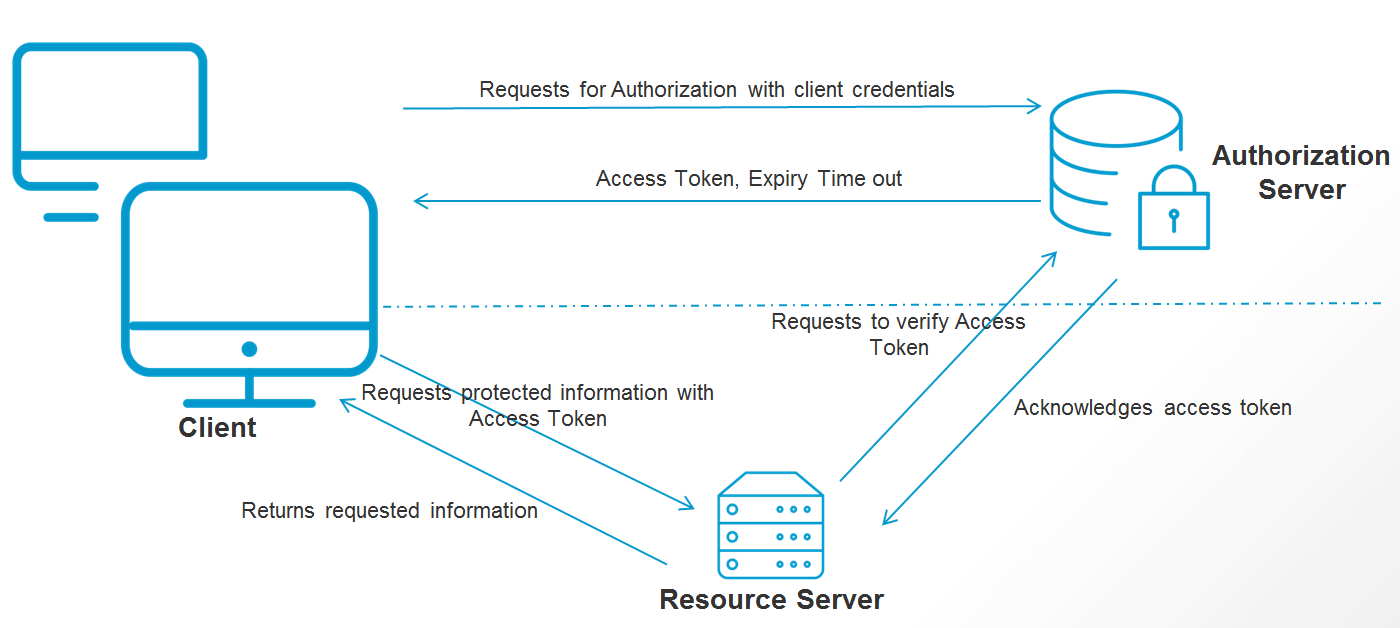
\includegraphics[width=0.8\textwidth]{BAB_TESIS/IMAGES/m2m_auth.png}
    \caption{Skema M2M Authentication}
    \label{fig:m2m}
\end{figure}

		\subsection{Metode Autentikasi Mesin ke Mesin}
		\label{metode autentikasi mesin ke mesin}
		Salah satu metode autentikasi Machine-to-Machine (M2M) menggunakan token merujuk pada proses verifikasi identitas antara dua atau lebih perangkat atau sistem tanpa intervensi manusia. Dalam skenario ini, token digunakan sebagai kredensial atau kunci otentikasi yang diberikan kepada perangkat atau sistem untuk membuktikan identitasnya kepada sistem yang lain.


			\subsubsection{\textit{Basic Access Authentication}}
			\label{basic access authentication}
			\input{BAB_TESIS/BAB3/3_3_1_BASIC_ACCESS_AUTHENTICATION}

			\subsubsection{\textit{Token}}
			\label{token}
			Klien membuat permintaan ke server otorisasi dengan mengirimkan ID klien, rahasia klien, bersama dengan audiens dan klaim-klaim lainnya. Server otorisasi memvalidasi permintaan tersebut, dan, jika berhasil, mengirimkan respons dengan token akses. Klien sekarang dapat menggunakan token akses untuk meminta sumber daya yang dilindungi dari server sumber daya.
Karena klien harus selalu menjaga rahasia klien, pemberian ini hanya dimaksudkan untuk digunakan pada klien terpercaya. Dengan kata lain, klien yang menyimpan rahasia klien harus selalu digunakan di tempat di mana tidak ada risiko rahasia tersebut disalahgunakan. Sebagai contoh, meskipun mungkin ide yang baik untuk menggunakan hibah kredensial klien di sistem internal yang mengirimkan laporan di seluruh web ke bagian lain dari sistem Anda, namun tidak dapat digunakan untuk alat publik yang dapat diakses oleh pengguna eksternal mana pun.
Berikut ini adalah permintaan HTTP yang relevan pada Tabel \ref{tab:req_http} berikut:

\begin{table}[H]
    \caption{Permintaan HTTP}
    \vspace{0.5em}
    \centering
    \begin{tabular}{|c|c|c|}
        \hline
        Permintaan & Deskripsi \\
        \hline \hline
        POST & Metode HTTP \\
        \hline
        /token & Endpoint \\
        \hline
        grant\_type=client\_credentials & Jenis hibah \\
        \hline
        & ID klien \\
        \hline
        & Rahasia klien \\
        \hline
        & Audiens \\
        \hline
    \end{tabular}
    \label{tab:req_http}
\end{table}

Sedangkan berikut contoh respon HTTP yang relevan pada Tabel \ref{tab:res_http} berikut:

\begin{table}[h]
    \caption{Respon HTTP}
    \vspace{0.5em}
    \centering
    \begin{tabular}{|c|c|c|}
        \hline
        Respon & Deskripsi \\
        \hline \hline
        200 OK & Kode status HTTP \\
        \hline
        Content-Type: application/json & Header HTTP \\
        \hline
        Cache-Control: no-store & Header HTTP \\
        \hline
        Pragma: no-cache & Header HTTP \\
        \hline
        \{ & Body \\
        \hline
        "access\_token": "2YotnFZFE & \\
        \hline
        "token\_type": "example", & \\
        \hline
        "expires\_in": 3600, & \\
        \hline
        "example\_parameter": "example\_value" & \\
        \hline
        \} & \\
        \hline
    \end{tabular}
    \label{tab:res_http}
\end{table}

	\section{\textit{Risk-Based Authentication}}
	\label{risk-based authentication}
	Risk-based adalah suatu metode yang digunakan untuk mengukur dan
mengelola risiko. Dalam konteks keamanan, risk-based authentication adalah metode autentikasi yang mengukur tingkat risiko dari suatu permintaan akses, dan mengambil tindakan yang sesuai berdasarkan tingkat risiko tersebut. Metode ini bertujuan untuk mengenali dan menangani ancaman potensial tanpa mengekang fleksibilitas dan kenyamanan pengguna.
Dalam konteks Machine-to-Machine (M2M) authentication, risk-based authentication digunakan untuk mengukur tingkat risiko dari suatu permintaan akses dan mengambil tindakan yang sesuai berdasarkan tingkat risiko tersebut.
Prosesnya dapat dilakukan dengan cara menganalisis faktor-faktor yang dapat meningkatkan risiko, seperti lokasi geografis, waktu akses, dan jenis perangkat yang digunakan.
Setelah tingkat risiko diukur, sistem dapat mengambil tindakan yang sesuai. Jika tingkat risiko dianggap rendah, maka autentikasi dapat dilakukan secara otomatis tanpa intervensi manusia. Namun, jika tingkat risiko dianggap tinggi, maka autentikasi dapat dilakukan dengan cara yang lebih ketat, seperti mengharuskan verifikasi melalui kode SMS atau panggilan telepon, atau pembatasan akses sesuai dengan level risiko.
Risk-based authentication juga dapat digabungkan dengan metode analisis risiko dinamis, yaitu mengukur risiko secara real-time dan mengambil tindakan sesuai dengan situasi yang ada. Ini dapat membantu sistem untuk mengenali dan menangani ancaman potensial secara efektif tanpa mengekang fleksibilitas dan kenyamanan pengguna seperti ilustrasi pada Gambar 3.2.

Bagian ini membahas pertimbangan etis penelitian dan potensi masalah serta
keterbatasannya. Jika menyangkut penelitian dengan makhluk hidup, maka dibutuhkan adanya \textit{ethical clearance}, di bagian ini hal itu akan dibahas. Demikian juga tentang keterbatasan ataupun masalah yang akan timbul.

	\section{\textit{Classification and Regression Tree (CART)}}
	\label{classification and regression tree}
	Metode CART merupakan suatu metode pohon keputusan (decision tree) yang bersifat recursive partitioning. Satu tree terdiri atas tiga komponen utama yaitu root node, internal node dan terminal node. Pada metode CART simpul akar (root node) dipartisi menjadi dua simpul anak (internal node), masing-masing simpul anak kemudian dipartisi menjadi dua simpul anak yang baru hingga menjadi terminal node yang bersifat homogen sebagai interpretasi dari tree Zhang, H \& Singer (2010). CART membentuk tree dengan dua langkah yaitu, pembentukan maksimal dari decision tree berdasarkan proses splitting (pemilahan) dan pemangkasan (pruning) dengan mempertimbangkan tree dan cabang pohon yang terbentuk. Proses splitting variabel pada percabangan node pada tree dilihat dari variabel yang memiliki nilai goodness of split maksimal. Nilai ini dilihat berdasarkan perubahan gini impurity/gini index pada node t dan percabangan nodenya menurut Gordon dkk. (1984) dengan rumus sebagai berikut.
%insert equation
\\
Node Kiri:
\begin{equation}
    \text{imp}(\mathbf{t}_{\text{L}}) = \sum_{l=1}^{2} p_{\text{tL}}(l)(1 - p_{\text{tL}}(l))
\end{equation}
\\
Node Kanan:
\begin{equation}
    \text{imp}(\mathbf{t}_{\text{R}}) = \sum_{l=1}^{2} p_{\text{tR}}(l)(1 - p_{\text{tR}}(l))
    \end{equation}
\\ 
Node t:
\begin{equation}
    \text{imp}(\mathbf{t}) = \sum_{k=1}^{2} p_{\text{t}}(k)(1 - p_{\text{t}}(k))
    \end{equation}
\\
Keterangan:
\begin{equation}
    p_{t}(k) = \frac{n_{t}(k)}{n_{t}} \quad \text{dan} \quad p_{t}(l) = \frac{n_{t}(l)}{n_{t}}
    \end{equation}
\\
\begin{equation}
    p_{t}(k), p_{t}(l) : \text{Proporsi objek kelas klasifikasi ke-} k \text{ atau ke-} l \text{ pada node } t
    \end{equation}
    
    \begin{equation}
    n_{t}(k), n_{t}(l) : \text{Jumlah observasi kelas klasifikasi ke-} k \text{ atau ke-} l \text{ pada node } t
    \end{equation}
    
    \begin{equation}
    n_{t} : \text{Jumlah seluruh observasi pada node } t
    \end{equation}

		\subsection{\textit{Random Forest}}
		\label{random forest}
		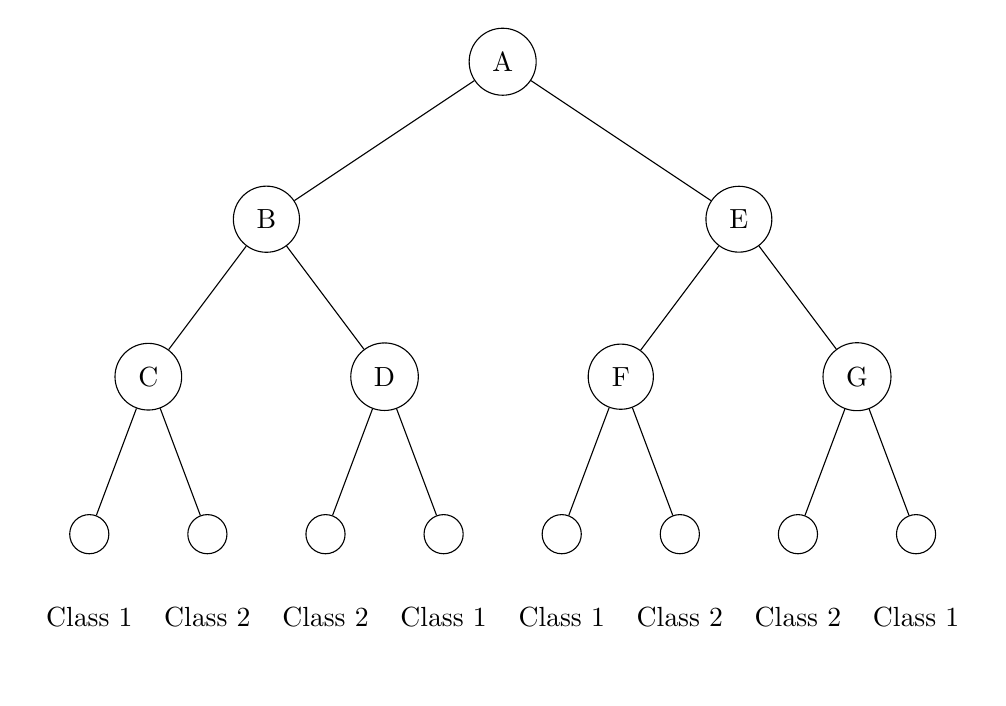
\begin{tikzpicture}[
    grow=down,
    level 1/.style={sibling distance=6cm, level distance=2cm},
    level 2/.style={sibling distance=3cm, level distance=2cm},
    level 3/.style={sibling distance=1.5cm, level distance=2cm},
    every node/.style={draw, circle, inner sep=0.5em}
  ]
  
  % Root node
  \node {A}
    child {
      node {B}
      child {
        node {C}
        child {node[label=below:Class 1] {}}
        child {node[label=below:Class 2] {}}
      }
      child {
        node {D}
        child {node[label=below:Class 2] {}}
        child {node[label=below:Class 1] {}}
      }
    }
    child {
      node {E}
      child {
        node {F}
        child {node[label=below:Class 1] {}}
        child {node[label=below:Class 2] {}}
      }
      child {
        node {G}
        child {node[label=below:Class 2] {}}
        child {node[label=below:Class 1] {}}
      }
    };
  
  \end{tikzpicture}

Membentuk tree lainnya sehingga terbentuk beberapa tree berdasarkan ntree Random Forest (RF) merupakan pengembangan metode CART. RF merupakan kumpulan banyak decision tree untuk membangun satu forest dan melihat vote klasifikasi dari tree yang menghasilkan prediktif lebih akurat Genuer dkk. (2008). Tree di RF dibentuk tidak menggunakan seluruh sampel melainkan menggunakan sampel bootstrap dan tidak melakukan pruning. Bootstrap merupakan metode berbasis resampling data dengan syarat pengembalian dalam menyelesaikan suatu permasalahan James dkk. (2021). Pada RF sampel bootstrap yang digunakan adalah 2/3 data original dengan pengembalian sehingga membentuk sampel bootstrap yang memiliki jumlah sama dengan data original sedangkan 1/3 data original lainnya disebut sampel out of bag (OOB) yang digunakan untuk pengujian prediksi tree yang sudah terbentuk dari sampel bootstrap Breiman (2001).
Terdapat tiga tuning parameter yang digunakan metode RF yaitu mtry (banyak input variabel secara acak terpilih dalam satu node pemilahan) yang secara default mtry = $\sqrt{p}$ untuk kasus klasifikasi, ntree (jumlah banyaknya tree dalam forest) yang secara default ntree = 500, penelitian ini menggunakan ntree berjumlah 100, 250, 500, dan 1000, serta node size (minimum nomor observasi dalam sebuah node) yang secara default 1 untuk klasifikasi Probst dkk. (2019). Pembentukan tree pada RF dilakukan dengan cara membentuk sampel bootstrap, lalu melakukan teknik recursive partitioning pada sampel bootstrap sehingga menghasilkan sebuah tree, dimana dalam proses splitting tree atribut diambil berdasarkan banyaknya variabel yang terpilih melalui mtry. Selanjutnya, melakukan kembali pembentukan sampel bootstrap dan metode recursive partitioning untuk dalam membangun satu forest untuk melihat vote klasifikasi dari seluruh tree yang terbentuk.


		\subsection{Laju Galat klasifikasi}
		\label{laju galat klasifikasi}
		OOB sampel berfungsi sebagai percobaan prediksi tree yang terbentuk dikarenakan setiap tree memiliki sampel bootstrap yang berbeda, sehingga setiap amatan dapat menjadi sampel OOB dan perlu diprediksi menggunakan beberapa tree yang dibangun tidak menggunakan sampel tersebut. Estimasi error pada hasil prediksi RF dapat diduga dengan menggunakan laju galat OOB (OOB error rate) yang dihitung dari hasil proporsi kesalahan prediksi klasifikasi setiap amatan dari hasil RF Janitza \& Hornung (2018). Penggunaan mtry untuk melihat hasil dari OOB error diharapkan tidak terlalu rendah, dikarenakan apabila terlalu rendah, maka hasil OOB error akan semakin tinggi yang menghasilkan RF memiliki kinerja yang buruk. OOB error rate diharapkan memiliki nilai terkecil (minimum). Berikut perhitungan laju galat OOB dalam klasifikasi.

\begin{equation}
    \text{Laju Galat } \text{OOB}_i = \frac{1}{n} \sum_{i=1}^{n} \mathbb{I}(Y_i \neq P_i)
    \end{equation}

OOB error rate digunakan untuk memprediksi observasi ke- $i$ dari $Xi$ dimana
prediksi hanya berlaku untuk suatu tree yang sampel bootstrapnya tidak mengandung ($Xi$, $Yi$)
    

		\subsection{\textit{Variable Importance Measure(VIM)}}
		\label{variable importance measure}
		Penggunaan analisis dalam RF secara umum sangat sulit untuk melakukan interpretasi dalam memperoleh informasi. Salah satu solusi untuk mempermudah memperoleh informasi dalam RF ialah dengan mengidentifikasi Variable Importance Measure (VIM) untuk variabel prediktor. Apabila variabel importance dapat diidentifikasi, maka hasil RF akan diperoleh metode penyeleksian variabel yang berpengaruh penting terhadap pembentukan tree dalam RF. Estimasi pemilihan variabel importance dalam random forest dapat dilakukan dengan melihat berapa banyak kenaikan prediksi error (OOB) data untuk variabel terpilih sementara yang lainnya tidak berubah Liaw \& Wiener (2002).
Metode representatif dari perhitungan pengukuran variabel importance adalah Mean Decrease Impurity (MDI) atau disebut juga dengan Mean Decrease Gini (MDG) yang diusulkan oleh Breiman pada tahun 2001. Suatu p peubah penjelas dengan h=(1,2,…,p) maka rumus mengukur tingkat kepentingan peubah penjelas Xh dengan cara berikut (Xiao Li. dkk, 20 19).
\begin{equation}
  \text{MDG}(\mathbf{x}_h) = \frac{1}{k} \sum_{t=1}^{k} \text{MDG}(\mathbf{X}_h, \mathbf{x}_t)
  \end{equation}
\\
Keterangan:
\begin{equation}
  \text{MDG}(\mathbf{X}_h, \mathbf{x}_t) = \sum_{t \in (T), v(t) = h} \frac{N_n(t)}{n} \Delta\mathbf{x}(t)
  \end{equation}

  Selain itu, perhitungan VIM dapat juga dengan menggunakan perhitungan
  Mean Decrease Accuracy (MDA) atau Permutation Importance yang menggunakan
  OOB untuk membagi data sampelnya, dimana OOB memperkirakan nilai prediksi
  dengan menghitung nilai akurasi OOB sebelum dan sesudah permutasi Xh dan
  menghitung perbedaannya, dengan rumus sebagai berikut Strobl dkk. (2008)

  \begin{equation}
    \text{MDA}(\mathbf{x}_h) = \frac{1}{k} \sum_{t=1}^{k} \sum_{i \in \text{OOB}(t)} \frac{I(y_i = \hat{y}_i(t)) - I(y_i = \hat{y}_i, h(t))}{|\text{OOB}(t)|}
    \end{equation}

    dimana $OOB(t)$ adalah sampel $OOB$ untuk satu tree ke- $t$ , dengan t elemen dari 
{1,2,3, … , k}, tingkat kepentingan variabel Xh dalam tree ke $- t$ adalah nilai rata-
rata dari perbedaan antara kelas prediksi sebelum permutasi Xh yaitu $\hat{y}_i(t) = f(t)(x_i)$ dan kelas prediksi setelah permutasi Xh, yaitu $\hat{y}_{i,h}(t) = f(t)(x_{i,h})$
dalam $i$ observasi tertentu.

		\subsection{Metriks dan \textit{Scoring}}
		\label{metriks dan scoring}
		Ada beberapa cara untuk mengukur kinerja pengklasifikasi, tetapi yang paling umum adalah menggunakan matriks kebingungan, presisi, recall, dan skor F1.

\textit{Confusion matrix} atau dikenal juga dengan matriks kebingungan adalah cara untuk mengekspresikan berapa banyak prediksi pengklasifikasi yang benar, dan ketika salah, di mana pengklasifikasi mengalami kebingungan (sesuai dengan namanya). 
Pada matriks kebingungan di bawah ini, baris mewakili label yang benar dan kolom mewakili label yang diprediksi. Nilai pada diagonal mewakili jumlah (atau persen, dalam matriks kebingungan yang dinormalisasi) dari waktu di mana label yang diprediksi cocok dengan label yang sebenarnya. 
Nilai di sel lainnya mewakili contoh di mana pengklasifikasi salah memberi label pada pengamatan; kolom memberi tahu kita apa yang diprediksi oleh pengklasifikasi, dan baris memberi tahu kita apa label yang benar.

Presisi adalah jumlah anggota kelas yang diidentifikasi dengan benar dibagi dengan semua kali model memprediksi kelas tersebut. Dalam kasus Aspens, skor presisi adalah jumlah Aspens yang diidentifikasi dengan benar dibagi dengan jumlah total kali pengklasifikasi memprediksi Aspen, baik benar maupun salah.

Recall adalah jumlah anggota kelas yang diidentifikasi dengan benar oleh pengklasifikasi dibagi dengan jumlah total anggota dalam kelas tersebut. Untuk Aspen, ini adalah jumlah Aspen aktual yang diidentifikasi dengan benar oleh pengklasifikasi.

Skor F1 sedikit kurang intuitif karena menggabungkan presisi dan recall ke dalam satu metrik. Jika presisi dan recall keduanya tinggi, F1 juga akan tinggi. 
Jika keduanya rendah, F1 akan rendah. Jika salah satunya tinggi dan yang lainnya rendah, F1 akan rendah. F1 adalah cara cepat untuk mengetahui apakah pengklasifikasi benar-benar baik dalam mengidentifikasi anggota kelas, atau apakah pengklasifikasi menemukan jalan pintas (misalnya, hanya mengidentifikasi segala sesuatu sebagai anggota kelas yang besar).

	

%-----------------------------------------------------------------
% Akhir BAB 3
%-----------------------------------------------------------------


%-----------------------------------------------------------------
% Awal BAB 4
%-----------------------------------------------------------------
\chapter{ANALISIS DAN PERANCANGAN SISTEM}
\label{ANALISIS DAN PERANCANGAN SISTEM}

	\section{Deskripsi Umum Sistem}
	\label{rancangan deskripsi umum sistem}
	Analisis sistem terdiri dari gambaran umum sistem yang dapat dilihat pada Gambar \ref{fig:gambaran-umum}, deskripsi sistem, dan diagram alir sistem. Gambaran umum sistem menjelaskan secara singkat tentang sistem yang akan dibangun. Deskripsi sistem menjelaskan tentang sistem yang akan dibangun secara rinci. Diagram alir sistem menjelaskan tentang alur kerja sistem yang akan dibangun.

\begin{figure}[H]
    \centering
    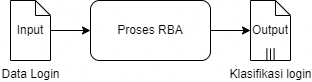
\includegraphics[width=0.6\textwidth]{BAB_TESIS/IMAGES/gambaran-umum.png}
    \caption{Gambaran Umum Sistem}
    \label{fig:gambaran-umum}
\end{figure}



	\section{Analisis Kebutuhan Sistem}
	\label{rancangan analisis kebutuhan sistem}
	Dalam membangun sistem ini, diperlukan analisa kebutuhan fungsional. Kebutuhan fungsional adalah kebutuhan yang berkaitan dengan fungsi-fungsi
yang harus ada dalam sistem. Serta akan dijelaskan kebutuhan perangkat keras dan perangkat lunak yang dibutuhkan dalam membangun sistem ini.

		\subsection{Analisis Kebutuhan Fungsional}
		\label{rancangan kebutuhan fungsional}
		Kebutuhan fungsional sistem ini adalah sebagai berikut:
\begin{enumerate}
    \item Sistem dapat melakukan analisis risiko autentikasi dengan menggunakan metode Random Forest.
    \item Sistem dapat men-genrate token autentikasi dari input user id.
    \item Sistem risiko autentikasi dapat terintegrasi dengan sistem FHIR.
\end{enumerate}

		\subsection{Analisis Kebutuhan Perangkat Keras}
		\label{rancangan analisis kebutuhan perangkat keras}
		\begin{enumerate}
    \item Laptop atau PC dengan RAM minimal 8gb.
    \item Prosessor dengan minimum 5 CPU Core.
    \item \textit{Storage} dengan minimum 50gb.
    \item Sistem operasi dengan base unix untuk menjalankan sistem klasifikasi.
\end{enumerate}

		\subsection{Analisis Kebutuhan Perangkat Lunak}
		\label{rancangan analisis kebutuhan perangkat lunak}
		\begin{enumerate}
    \item Bahasa pemrograman python versi 3.9 dengan \textit{framework} anaconda 3
    \item \textit{Framework} flask untuk membuat endpoint 
    \item Sistem operasi dengan base unix untuk menjalankan sistem klasifikasi
\end{enumerate}

	\section{Rancangan Sistem}
	\label{rancangan sistem}
	Berikut adalah rancangan sistem yang akan dibangun. Rancangan sistem terdiri dari rancangan arsitektur sistem, rancangan pembersihan data, rancangan variabel kepentingan, dan rancangan integrasi dengan sistem FHIR.


		\subsection{Rancangan Arsitektur Sistem}
		\label{rancangan Arsitektur Sistem}
		Rancangan arsitektur sistem dapat dilihat pada Gambar \ref{fig:arsitektur-sistem}. Sistem ini terdiri dari 3 komponen utama yaitu komponen \textit{data preprocessing}, komponen \textit{data mining}, dan komponen \textit{data integration}. Komponen \textit{data preprocessing} berfungsi untuk membersihkan data dari \textit{noise} dan \textit{outlier}. Komponen \textit{data mining} berfungsi untuk melakukan analisis risiko autentikasi dengan menggunakan metode Random Forest. Komponen \textit{data integration} berfungsi untuk mengintegrasikan sistem dengan sistem FHIR.

\begin{figure}[H]
    \centering
    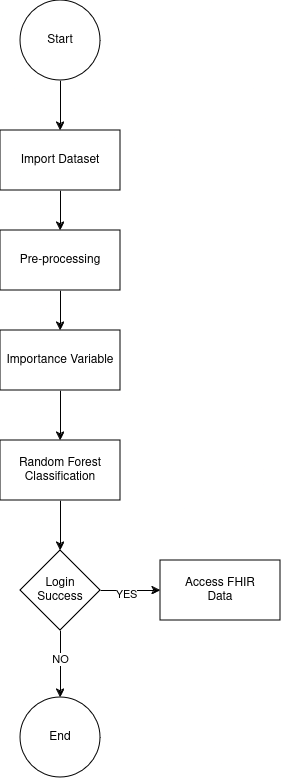
\includegraphics[width=0.5\textwidth]{BAB_TESIS/IMAGES/diagram_kusus.drawio.png}
    \caption{Rancangan Arsitektur Sistem}
    \label{fig:arsitektur-sistem}
\end{figure}

Pada Gambar \ref{fig:arsitektur-sistem}, sistem ini akan mendapatkan data login dari datasest. Data login ini kemudian akan digunakan sebagai input untuk melakukan analisis risiko autentikasi. Dalam menentukan risiko autentikasi, sistem ini akan menggunakan metode Random Forest. Metode Random Forest akan menghasilkan variabel kepentingan yang dapat digunakan untuk melakukan analisis risiko autentikasi.

Setelah itu, sistem ini akan terintegrasi dengan sistem FHIR. Sistem ini akan menggunakan FHIR API untuk mengakses data dari sistem FHIR. FHIR API akan mengakses data dari sistem FHIR dengan menggunakan \textit{request} dan \textit{response}.

		\subsection{Rancangan Pembersihan Data}
		\label{rancangan pembersihan data}
		Rancangan pembersihan data dapat dilihat pada Gambar \ref{fig:pembersihan-data} Pada tahap ini, data akan dibersihkan dari \textit{noise} dan \textit{outlier}. \textit{Noise} adalah data yang tidak memiliki nilai yang berarti. \textit{Outlier} adalah data yang memiliki nilai yang ekstrim. Pada tahap ini, data akan dibersihkan dari \textit{noise} dan \textit{outlier} dengan menggunakan beberapa metode yaitu :

\begin{figure}[H]
    \centering
    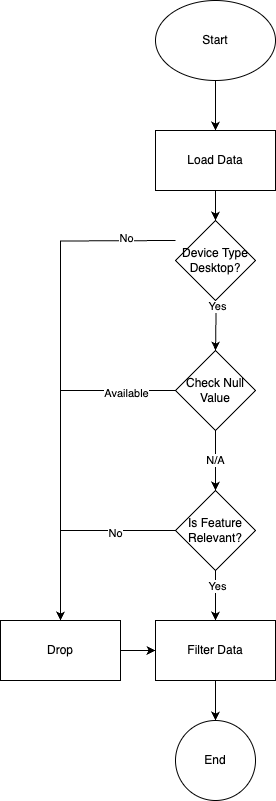
\includegraphics[width=0.4\textwidth]{BAB_TESIS/IMAGES/pre-processing.png}
    \caption{Rancangan Pembersihan Data}
    \label{fig:pembersihan-data}
\end{figure}

Dalam melakukan pembersihan data, sistem ini akan dua metode yaitu :

\begin{enumerate}
    \item \textit{Missing Value} : Menghapus data yang memiliki nilai kosong.
    \item \textit{Duplicate Elimination} : Menghapus duplikasi data sehingga hanya satu dari data duplikat yang disimpan. 
\end{enumerate}

Pembersihan tahap satu dapat dilakukkan menggunakan fitur pandas yaitu isnull. Setelah itu didapatkan jumlahnya dengan sum. Dengan cara ini didapatkan jumlah data kosong untuk setiap fitur. Untuk fitur yang terdapat nilai kosong akan dibuang
Pembersihan tahap dua dilakukkan dengan cara menyaring fitur \textit{User Agent and Device Type} 
Setelah data dibersihkan, data akan digunakan sebagai input untuk melakukan analisis risiko autentikasi. Data ini kemudian akan digunakan sebagai input untuk melakukan analisis risiko autentikasi.

		% masukkan rancangan split data 70-30

		\subsection{Rancangan \textit{Encoding}}
		\label{rancangan encoding}
		One-hot encoding adalah teknik pengkodean kategoris yang umum digunakan dalam pemrosesan data. Mengkutip dari James, G, et al. (2013) teknik ini cocok untuk variabel kategori di mana kategori tidak memiliki urutan atau hubungan yang melekat dengan nilai numeriknya. Ide di balik pengkodean one-hot adalah untuk mewakili setiap kategori sebagai vektor biner yang panjangnya sama dengan jumlah kategori unik dalam variabel tersebut.

\begin{table}[htbp]
    \caption{Sample Encoding Data}
    \centering
    \resizebox{\textwidth}{!}{%
    \begin{tabular}{|c|c|c|c|c|c|c|c|c|}
    \hline
    login\_timestamp\_1 & login\_timestamp\_2 & ip\_address\_1 & ip\_address\_2 & country\_1 & country\_2 & region\_1 & region\_2 & city\_1 \\ \hline
    0 & 1 & 0 & 1 & 0 & 1 & 0 & 1 & 0 \\ \hline
    1 & 0 & 1 & 0 & 1 & 0 & 1 & 0 & 1 \\ \hline
    \end{tabular}%
    }
    \label{tab:sample_table}
\end{table}


Cara kerja one-hot encoding adalah seperti ditunjukan pada Tabel \ref{tab:sample_table} dengan membuat kolom biner baru untuk setiap kategori dalam kolom kategori. Jika terdapat N kategori unik, maka akan dibuat N kolom biner baru. 
Setiap kolom biner akan memiliki nilai 1 jika kategori tersebut hadir dalam observasi, dan nilai 0 jika tidak hadir. Dengan demikian, setiap observasi direpresentasikan sebagai vektor biner dengan panjang N, di mana setiap elemen vektor menunjukkan keberadaan atau ketiadaan kategori yang sesuai dalam observasi. Teknik ini memungkinkan model machine learning untuk memahami dan memproses variabel kategori dalam bentuk yang sesuai dengan algoritma yang digunakan, seperti algoritma regresi logistik atau jaringan saraf.

Meskipun memiliki kelebihan, One-Hot Encoding juga memiliki beberapa kekurangan signifikan. Salah satu kekhawatiran utama adalah potensi untuk menghasilkan data berdimensi tinggi. Untuk fitur kategorikal dengan banyak nilai unik, One-Hot Encoding dapat menghasilkan sejumlah besar fitur biner, yang dapat meningkatkan biaya komputasi dan risiko overfitting. Masalah ini terutama terlihat pada dataset dengan kardinalitas tinggi, di mana jumlah fitur biner yang baru dapat menjadi sangat banyak. Selain itu, peningkatan dimensi dapat menyebabkan penggunaan memori yang lebih tinggi, terutama dalam dataset besar dengan banyak variabel kategorikal. Kebutuhan memori tambahan ini dapat mempengaruhi kecepatan dan efisiensi proses pelatihan.


		\subsection{Rancangan \textit{Variable Importance Measure}}
		\label{rancangan variable importance measure}
		Rancangan variabel kepentingan akan dilakukan dengan menggunakan metode Random Forest. Metode Random Forest akan menghasilkan variabel kepentingan yang dapat dilihat pada Gambar \ref{fig:variabel-kepentingan}. Variabel kepentingan ini akan digunakan untuk melakukan analisis risiko autentikasi.
Berikut adalah rancangan variabel kepentingan yang akan digunakan untuk melakukan analisis risiko autentikasi.
\begin{figure}[H]
    \centering
    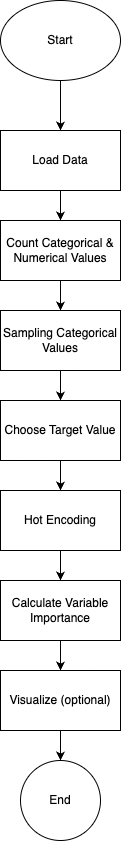
\includegraphics[width=0.2\textwidth]{BAB_TESIS/IMAGES/vim.drawio.png}
    \caption{Rancangan Variabel Kepentingan}
    \label{fig:variabel-kepentingan}
\end{figure}

Gambar \ref{fig:variabel-kepentingan} menjelaskan bahwa variabel kepentingan akan digunakan untuk melakukan analisis risiko autentikasi. Variabel kepentingan ini akan digunakan sebagai input untuk melakukan analisis risiko autentikasi.
Setelah data berhasil di-import akan diakukan penghitungan kategorikal dan numerikal data. 

		\subsection{Rancangan Integrasi Sistem FHIR}
		\label{rancangan integrasi sistem fhir}
		Rancangan integrasi dengan sistem FHIR dapat dilihat pada Gambar 4.6. Sistem ini akan terintegrasi dengan sistem FHIR untuk mendapatkan data login dari pasien. Data login ini kemudian akan digunakan sebagai input untuk melakukan analisis risiko autentikasi.
\begin{figure}[H]
    \centering
    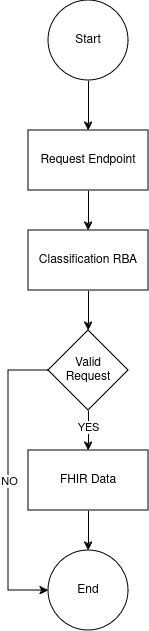
\includegraphics[width=0.2\textwidth]{BAB_TESIS/IMAGES/fhir_rba.drawio.png}
    \caption{Rancangan Integrasi Dengan Sistem FHIR}
    \label{fig:integrasi}
\end{figure}

Gambar \ref{fig:integrasi} dijelaskan proses penggunaan model prediksi Random Forest dengan API, dan bagaimana permintaan data FHIR (Fast Healthcare Interoperability Resources) diproses. Proses dimulai dengan menerima permintaan (Request Endpoint) dari pengguna untuk memperoleh prediksi. Setelah menerima permintaan, sistem kemudian melakukan klasifikasi RBA (Risk-Based Authentication), sebuah langkah untuk mengidentifikasi dan mengevaluasi risiko terkait permintaan tersebut.

Pada tahap berikutnya, sistem mengevaluasi validitas permintaan melalui titik keputusan (Valid Request). Jika permintaan tersebut valid, maka data FHIR yang diminta akan dikirimkan (FHIR Data) dan proses berakhir. Namun, jika permintaannya tidak valid, proses dihentikan tanpa mengakses data FHIR.

Dalam konteks ini, API schema berikut menjelaskan struktur yaml yang digunakan untuk melakukan permintaan prediksi menggunakan model Random Forest:

\begin{lstlisting}
    tags:
      - Prediction
    parameters:
      - name: body
        in: body
        required: true
        schema:
          type: object
          required:
            - features
            - patient_id
          properties:
            features:
              type: array
              items:
                type: number
              example: [5.1, 3.5, 1.4, 0.2]
            patient_id:
              type: string
              example: "example_patient_id"
    responses:
      200:
        description: Prediction result
        schema:
          type: object
          properties:
            prediction:
              type: integer
              example: 1
            observation:
              type: object
      400:
        description: Bad Request
        schema:
          type: object
          properties:
            error:
              type: string
              example: Missing features key in the JSON data
      500:
        description: Internal Server Error
        schema:
          type: object
          properties:
            error:
              type: string
              example: Internal error message
    \end{lstlisting}

    Schema yaml tersebut digunakan dalam permintaan untuk prediksi dengan Random Forest Model. Permintaan ini harus menyertakan dua parameter penting: \texttt{features} dan \texttt{patient\_id}. Parameter \texttt{features} adalah array berisi nilai numerik yang akan digunakan model untuk prediksi, sementara \texttt{patient\_id} adalah string pengidentifikasi pasien yang bersangkutan. Respon yang diberikan oleh API memiliki format JSON yang mencakup hasil prediksi (\texttt{prediction}) dan observasi tambahan (\texttt{observation}), atau deskripsi kesalahan jika terjadi kesalahan saat pemrosesan.

    Secara keseluruhan, diagram dan schema ini menjelaskan alur proses yang harus diikuti untuk melakukan prediksi menggunakan Random Forest Model dan mengakses data FHIR, yang diawali dari penerimaan permintaan hingga penyediaan hasil atau tanggapan kesalahan. Pendekatan ini memastikan adanya langkah-langkah yang terstruktur dan aman dalam pengelolaan serta pemanfaatan data.
    

	\section{Rancangan Pengujian}
	\label{rancangan pengujian}
	Pengujian sistem ini akan dilakukan dengan menggunakan beberapa metode yaitu:
\begin{enumerate}
    \item Pengujian Fungsional : Pengujian fungsional dilakukan untuk menguji apakah sistem dapat berjalan dengan baik sesuai dengan kebutuhan fungsional yang telah ditentukan.
    \item Menentukan Evaluasi : Akurasi, Presisi, \textit{Recall}, \textit{F1 Score}, dan \textit{Confusion Matrix} akan digunakan untuk menentukan evaluasi dari sistem.
    \item Membandingkan dengan autentikasi heuristik lainnya
\end{enumerate}


%-----------------------------------------------------------------
% Akhir BAB 4
%-----------------------------------------------------------------


%-----------------------------------------------------------------
% Awal BAB 5
%-----------------------------------------------------------------

\chapter{IMPLEMENTASI SISTEM}
\label{IMPLEMENTASI SISTEM}
Pada bab ini akan dijelaskan mengenai implementasi dari sistem yang telah dibangun. Implementasi sistem ini terdiri dari pengumpulan data, persiapan data, pemilihan fitur, dan pembangunan sistem.


	\section{Pengumpulan Data}
	\label{implementasi pengumpulan data}
	Dalam penelitian ini data yang digunakan adalah data fitur login dari lebih dari 33 juta upaya login dan lebih dari 3,3 juta pengguna pada layanan online berskala besar di Norwegia. Data asli dikumpulkan antara Februari 2020 dan Februari 2021 dari Kaggle. Data ini berisi 284807 baris data dengan 31 kolom. Kolom-kolom tersebut adalah sebagai berikut:

\begin{longtable}{|p{0.2\textwidth}|p{0.15\textwidth}|p{0.3\textwidth}|p{0.2\textwidth}|}
    \hline
    \textbf{Feature} & \textbf{Data Type} & \textbf{Description} & \textbf{Range or Example} \\ \hline
    IP Address & String & IP address belonging to the login attempt & 0.0.0.0 - 255.255.255.255 \\ \hline
    Country & String & Country derived from the IP address & US \\ \hline
    Region & String & Region derived from the IP address & New York \\ \hline
    City & String & City derived from the IP address & Rochester \\ \hline
    ASN & Integer & Autonomous system number derived from the IP address & 0 - 600000 \\ \hline
    User Agent String & String & User agent string submitted by the client & Mozilla/5.0 (Windows NT 10.0; Win64; ... \\ \hline
    OS Name and Version & String & Operating system name and version derived from the user agent string & Windows 10 \\ \hline
    Browser Name and Version & String & Browser name and version derived from the user agent string & Chrome 70.0.3538 \\ \hline
    Device Type & String & Device type derived from the user agent string & (`mobile`, `desktop`, `tablet`, `bot`, `unknown`) \\ \hline
    User ID & Integer & Identification number related to the affected user account & Random pseudonym \\ \hline
    Login Timestamp & Integer & Timestamp related to the login attempt & 64 Bit timestamp \\ \hline
    Round-Trip Time (RTT) [ms] & Integer & Server-side measured latency between client and server & 1 - 8600000 \\ \hline
    Login Successful & Boolean & `True`: Login was successful, `False`: Login failed & (`true`, `false`) \\ \hline
    Is Attack IP & Boolean & IP address was found in known attacker data set & (`true`, `false`) \\ \hline
    Is Account Takeover & Boolean & Login attempt was identified as account takeover by incident response team of the online service & (`true`, `false`) \\ \hline
    \caption{Deskripsi tabel fitur login}
    \label{tab:my_label}
\end{longtable}

	\section{\textit{Preprocessing Data}}
	\label{implementasi preprocessing data}
	Penggunaan dataset dalam penelitian ini membutuhkan beberapa tahapan persi-
apan data, yaitu pengumpulan data, pembersihan data, dan pemilihan fitur.

		\subsection{Eksplorasi Data}
		\label{implementasi eksplorasi data}
		Tahap ini diperlukan untuk mendapat gambaran umum mengenai data yang digunakan. Pada tahap ini dilakukan eksplorasi data untuk mengetahui jumlah baris dan kolom, tipe data, dan statistik deskriptif dari data. Hasil eksplorasi data dapat dilihat pada Tabel 5.1.


		\subsection{Pengecekan \textit{Missing Value}}
		\label{implementasi pengecekan missing value}
		Menggunakan kode berikut untuk mengecek apakah ada nilai yang hilang pada setiap kolom.
\begin{lstlisting}
    features.isnull().sum()
    \end{lstlisting}

hasilnya adalah sebagai berikut:

\begin{table}[H]
    \caption{Missing Values in Each Feature}
    \centering
    \begin{tabular}{|l|l|}
    \hline
    \textbf{Feature} & \textbf{Missing Values} \\ \hline
    Index & 0 \\ 
    Login Timestamp & 0 \\ 
    User ID & 0 \\ 
    Round-Trip Time [ms] & 29993329 \\ 
    IP Address & 0 \\ 
    Country & 0 \\ 
    Region & 47409 \\ 
    City & 8590 \\ 
    ASN & 0 \\ 
    User Agent String & 0 \\ 
    Browser Name and Version & 0 \\ 
    OS Name and Version & 0 \\ 
    Device Type & 1526 \\ 
    Login Successful & 0 \\ 
    Is Attack IP & 0 \\ 
    Is Account Takeover & 0 \\ \hline
    \end{tabular}
    \label{tab:missing_values}
    \end{table}

Dari tabel, terlihat bahwa sebagian besar kolom tidak memiliki nilai yang hilang, namun ada juga yang memilikinya. Misalnya, kolom 'Waktu Pulang Pergi [ms]' memiliki 29993329 nilai yang hilang, kolom 'Wilayah' memiliki 47409 nilai yang hilang, kolom 'Kota' memiliki 8590 nilai yang hilang, dan kolom 'Jenis Perangkat' memiliki 1526 nilai yang hilang.

		
		\subsection{Pemilihan Target}
		\label{implementasi pemilihan target}
		Pada tahap ini dilakukan pemilihan target yang akan diprediksi. Sebagaimana Random Forest merupakan algoritma klasifikasi, maka penelitian ini memerlukan fitur apa yang menjadi target.

Melakukkan sampling terhadap tiga kolom yang dapat menjadi target, yaitu 'Login Successful', 'Is Attack IP', dan 'Is Account Takeover'. Berikut adalah kode untuk sampling data.

\begin{lstlisting}
    # calculate the percentage of True and False values in bolean char'
    value_counts_1 = df['is_login_success'].value_counts(normalize=True)
    is_login_success_true = value_counts_1[True] * 100
    is_login_success_false = value_counts_1[False] * 100
    print("is_login_success")
    print(f"Percentage of True values: {is_login_success_true:.2f}%")
    print(f"Percentage of False values: {is_login_success_false:.2f}%")

    value_counts_2 = df['is_attack_ip'].value_counts(normalize=True)
    is_attack_ip_true  = value_counts_2[True] * 100
    is_attack_ip_false = value_counts_2[False] * 100
    print("is_attack_ip")
    print(f"Percentage of True values: {is_attack_ip_true:.2f}%")
    print(f"Percentage of False values: {is_attack_ip_false:.2f}%")

    value_counts_3 = df['is_account_takeover'].value_counts(normalize=True)
    is_account_takeover_true  = value_counts_3[True] * 100
    is_account_takeover_false = value_counts_3[False] * 100
    print("is_account_takeover")
    print(f"Percentage of True values: {is_account_takeover_true:.2f}%")
    print(f"Percentage of False values: {is_account_takeover_false:.2f}%")
\end{lstlisting}

    Berikut adalah hasil sampling data.

    \begin{table}[H]
        \caption{Hasil Sampling Data}
        \centering
        \begin{tabular}{|l|l|l|}
        \hline
        \textbf{Target} & \textbf{True} & \textbf{False} \\ \hline
        Login Successful & 67,35\% & 32,65\% \\ \hline
        Is Attack IP & 3,09\% & 96,91\% \\ \hline
        Is Account Takeover & 0,01\% & 99,99\% \\ \hline
        \end{tabular}
        \label{tab:sampling_data}
        \end{table}

        Dari hasil sampling data di atas, terlihat bahwa kolom 'Login Successful' memiliki persentase True yang lebih besar dibandingkan dengan False, sehingga kolom ini dipilih sebagai target.


		\subsection{Penambahan Kolom Token}
		\label{implementasi penambahan kolom token}
		Kolom token dibuat untuk menyimpan token yang digunakan untuk mengakses API. Kolom ini dibuat dengan cara mengenerate token secara acak menggunakan SHA512. Berikut adalah contoh kode untuk membuat kolom token.

\begin{lstlisting}
    # generate SHA512 Hash from user_id as m2m token
    import hashlib

    def generate_sha512_hash(user_id):
        sha512_hash = hashlib.sha512()
        sha512_hash.update(str(user_id).encode('utf-8'))
        return sha512_hash.hexdigest()

    features['token'] = features['user_id'].apply(generate_sha512_hash)
    \end{lstlisting}

Berikut adalah contoh token yang digenerate.

\begin{table}[H]
    \caption{Contoh Token}
    \begin{tabular}{|l|l|}
    \hline
    \textbf{User ID} & \textbf{Token} \\ \hline
    -3065936140549856249 & 4ffe29f1960c24624ec2c36909f3b39cb8d59fa18515f4 \\
    5932501938287412564 & ecee6cc95d3b047c8f796b8e772a468124b7ddb599a7a3 \\ \hline
    \end{tabular}
    \label{tab:token}
    \end{table}


	\section{Pembersihan Data}
	\label{implementasi pembersihan data}
	Pada proses pembersihan data, dilakukan penamaan kolom, pembersihan data yang tidak diperlukan, seperti kolom 'Index' dan lainnya. Berikut adalah contoh kode untuk melakukan pembersihan data.


		\subsection{Penamaan Kolom}
		\label{implementasi penamaan kolom}
		Penamaan kolom dilakukan untuk mempermudah pemanggilan kolom. Berikut adalah contoh kode untuk melakukan penamaan kolom.

\begin{lstlisting}
    # rename above columns to snake case
    features = features.rename(columns={'Login Timestamp': 'login_timestamp', 'User ID': 'user_id', 'Round-Trip Time [ms]':'round_trip','Region':'region', 'City':'city', 'ASN':'asn', 'IP Address': 'ip_address', 'Country': 'country', 'User Agent String': 'user_agent_string','Device Type': 'device_type', 'Browser Name and Version': 'browser', 'Is Account Takeover':'is_account_takeover', 'OS Name and Version':'os_detail','Login Successful':'is_login_success','Is Attack IP':'is_attack_ip'})
    \end{lstlisting}

    \begin{table}[H]
        \caption{Column Renaming in DataFrame}
        \centering
        \begin{tabular}{|l|l|}
        \hline
        \textbf{Original Column Name} & \textbf{New Column Name} \\ \hline
        Login Timestamp & login\_timestamp \\ 
        User ID & user\_id \\ 
        Round-Trip Time [ms] & round\_trip \\ 
        Region & region \\ 
        City & city \\ 
        ASN & asn \\ 
        IP Address & ip\_address \\ 
        Country & country \\ 
        User Agent String & user\_agent\_string \\ 
        Device Type & device\_type \\ 
        Browser Name and Version & browser \\ 
        Is Account Takeover & is\_account\_takeover \\ 
        OS Name and Version & os\_detail \\ 
        Login Successful & is\_login\_success \\ 
        Is Attack IP & is\_attack\_ip \\ \hline
        \end{tabular}
        \label{tab:column_renaming}
        \end{table}

		\subsection{Penyaringan Data}
		\label{implementasi penyaringan data}
		Hal ini dilakukan untuk membatasi jumlah dataset dan device type yang bertujuan mengurangi waktu komputasi dalam pembuatan model. Berikut adalah contoh kode untuk melakukan penyaringan user agent dan device type. 

\begin{lstlisting}
    # check lenght in column user_agent_string
    features['length'] = features['user_agent_string'].apply(
        lambda row: min(len(row), len(row)) if isinstance(row, str) else None
    )
    print(features['length'].mean())
    \end{lstlisting}

    Kode di atas digunakan untuk mengetahui panjang rata-rata string pada kolom 'User Agent String'. Hasilnya adalah 136.652141700553. 
    Setelah itu dilakukan penyaringan data dengan cara menghapus data yang memiliki panjang string lebih dari 136. Berikut adalah contoh kode untuk melakukan penyaringan data.

\begin{lstlisting}
    # only keep rows with device type desktop
    features = features[features.device_type == 'desktop']
    # filter the DataFrame based on the length of column 'user_agent_string'
    features = features[features['user_agent_string'].str.len() < 136]
    \end{lstlisting}

    Setelah itu dilakukan penyaringan data dengan cara menghapus data yang memiliki device type selain 'desktop'.


		\subsection{Penghapusan Kolom}
		\label{implementasi penghapusan kolom}
		Pada tahap ini dilakukan penghapusan kolom yang tidak diperlukan. Kolom yang dihapus adalah kolom 'Round-Trip Time [ms]', 'Index', 'Is Attack IP', 'Is Account Takeover', 'User ID', 'Token', 'Device Type', dan 'Length'. Berikut adalah contoh kode untuk menghapus kolom yang tidak diperlukan.

\begin{lstlisting}
    # drop unsued columns
    features = features.drop(['round_trip', 'index', 'is_attack_ip', 'is_account_takeover', 'user_id', 'token', 'device_type', 'length'], axis=1, inplace=True)
    \end{lstlisting}

Hasil keluaran dari tahap ini adalah sebagai berikut. 

\begin{table}[H]
	\caption{Revised Initial Exploratory Data Analysis}
    \centering
    \begin{tabular}{|l|l|l|l|}
    \hline
    \textbf{Column Name} & \textbf{Data Type} & \textbf{\#Distinct} & \textbf{NA Values} \\ \hline
    login\_timestamp & object & 30000 & 0 \\ 
    ip\_address & object & 17387 & 0 \\ 
    country & object & 75 & 0 \\ 
    region & object & 273 & 14 \\ 
    city & object & 1414 & 7 \\ 
    asn & int64 & 792 & 0 \\ 
    user\_agent\_string & object & 637 & 0 \\ 
    browser & object & 167 & 0 \\ 
    os\_detail & object & 61 & 0 \\ 
    is\_login\_success & bool & 2 & 0 \\ \hline
    \end{tabular}
    \label{tab:revised_initial_eda}
    \end{table}

    Berdasarkan tabel \ref{tab:revised_initial_eda}, diperoleh 30000 data, dengan 10 kolom, dan ada 14 data yang memiliki nilai kosong pada kolom 'Region' dan 7 data yang memiliki nilai kosong pada kolom 'City'.


	\section{Pemilihan Fitur Menggunakan \textit{Variable Importance Measure}}
	\label{implementasi pemilihan fitur menggunakan variable importance measure}
	Pada bagian ini akan dijelaskan mengenai implementasi pemilihan fitur. Pemilih-
an fitur dilakukan dengan cara memilih fitur yang memiliki korelasi tinggi dengan target.
Berikut adalah tahapan pemilihan fitur.

Sebelum itu dilakukan eksplorasi data untuk mengetahui jumlah baris dan kolom, tipe data, dan statistik deskriptif dari data. 
Tahap ini diperlukan untuk mengetahui tipe data dari setiap kolom. 

Asumsi yang digunakan adalah kolom yang memiliki tipe data numerik memiliki korelasi yang lebih tinggi dibandingkan dengan kolom yang memiliki tipe data string.
Berikut adalah contoh kode untuk mengetahui tipe data dari setiap kolom.

\begin{lstlisting}
    categorical = [var for var in df.columns if df[var].dtype=='O']
    print('There are {} categorical variables\n'.format(len(categorical)))
    print('The categorical variables are :\n\n', categorical)

    There are 8 categorical variables

    The categorical variables are :
    ['login_timestamp', 'ip_address', 'country', 'region', 'city', 'user_agent_string', 'browser', 'os_detail']
    \end{lstlisting}

    Berikut adalah hasil keluaran dari tahap ini.

    \begin{table}[H]
        \caption{Data Type of Each Column}
        \centering
        \begin{tabular}{|l|l|}
        \hline
        \textbf{Column Name} & \textbf{Data Type} \\ \hline
        login\_timestamp & object \\ 
        ip\_address & object \\ 
        country & object \\ 
        region & object \\ 
        city & object \\ 
        asn & int64 \\ 
        user\_agent\_string & object \\ 
        browser & object \\ 
        os\_detail & object \\ 
        is\_login\_success & bool \\ \hline
        \end{tabular}
        \label{tab:data_type}
        \end{table}

        Berdasarkan tabel \ref{tab:data_type}, terlihat bahwa kolom 'ASN' memiliki tipe data numerik, sedangkan kolom lainnya memiliki tipe data string.



			\subsection{\textit{Encoding Data}}
			\label{implementasi encoding data}
			Berdasarkan tabel di atas, terlihat bahwa kolom 'ASN' memiliki tipe data numerik, sedangkan kolom lainnya memiliki tipe data string. Oleh karena itu, perlu dilakukan encoding terhadap kolom-kolom yang memiliki tipe data string. Berikut adalah contoh kode untuk melakukan encoding.

\begin{lstlisting}
    import category_encoders as ce

    # One-hot encode the categorical features
    # encode categorical variables with ordinal encoding
    # see def preprocess_data(df) above
    encoder = ce.OneHotEncoder(cols= ['login_timestamp', 'ip_address', 'country', 'region', 'city', 'user_agent_string', 'browser', 'os_detail'])
    X_train = encoder.fit_transform(X_train)
    
    X_test = encoder.transform(X_test)
    X_train.head()
    \end{lstlisting}

Berikut adalah hasil keluaran dari tahap ini.

% to-do: add table here

			\subsection{\textit{Gini Importance}}
			\label{implementasi gini importance}
			Setelah dilakukan encoding, maka seluruh kolom memiliki tipe data numerik. Berikut adalah contoh kode untuk melakukan pemilihan fitur menggunakan Gini Importance.

\begin{lstlisting}
    ### Gini importance 
    # create the classifier with n_estimators = default
    clf = RandomForestClassifier(random_state=0)

    # fit the model to the training set
    clf.fit(X_train, y_train)

    # view the feature scores
    feature_scores = pd.Series(clf.feature_importances_, index=X_train.columns).sort_values(ascending=False)
    
    # Top 10 important features
    feature_scores.head(10) 
    \end{lstlisting}

    Pada kode di atas dilakukan pemilihan 10 fitur teratas. Dikarenakan jumlah fitur yang banyak, setelah dilakukkan encoding maka akan sulit untuk memvisualisasikan seluruh fitur.
    Berikut adalah hasil keluaran dari tahap ini.

    \begin{table}[H]
    \caption{Gini Importance of Each Feature}

    \centering
    \begin{tabular}{|l|l|}
    \hline
    \textbf{Feature} & \textbf{Gini Importance} \\ \hline
    asn & 0.017551 \\ 
    country\_2 & 0.009943 \\ 
    country\_4 & 0.004708 \\ 
    country\_6 & 0.003670 \\ 
    ip\_address\_23 & 0.003618 \\ 
    os\_detail\_1 & 0.003317 \\ 
    browser\_1 & 0.002975 \\ 
    os\_detail\_16 & 0.002832 \\ 
    user\_agent\_string\_49 & 0.002508 \\ 
    browser\_2 & 0.002213 \\ \hline
    \end{tabular}
    \label{tab:gini_importance}
    \end{table}

    Dalam tabel \ref{tab:gini_importance}, jika di lakukkan pengelompokkan maka akan terlihat bahwa fitur 'asn', 'country', 'ip\_address', 'os\_detail', 'browser', dan 'user\_agent\_string' memiliki nilai Gini Importance yang tinggi. 
    Namun, hanya 4 group teratas yang memiliki nilai Gini Importance yang tinggi, yaitu 'asn', 'country', 'ip\_address', dan 'os\_detail' yang akan digunakan sebagai fitur dalam pembuatan model.

	\section{Implementasi \textit{Random Forest}}
	\label{implementasi random forest}
	Pada bagian ini akan dijelaskan mengenai implementasi pembuatan Random Forest. Pembuatan Random Forest dapat dilakukan setelah memilih fitur yang memiliki korelasi tinggi dengan target. Berikut adalah tahapan pembuatan Random Forest.
Dari proses eksplorasi tipe data tabel 5.7 dan 5.2.2 pemilihan target, maka diperoleh bahwa kolom 'Login Successful' memiliki korelasi yang tinggi dengan target. Oleh karena itu, kolom ini dipilih sebagai target.

		\subsection{Pembagian Data}
		\label{implementasi pembagian data}
		Pada tahap ini dilakukan pembagian data fitur dan target. Berikut adalah contoh kode untuk melakukan pembagian data fitur dan target.
\begin{lstlisting}
    # Separate the features (X) and the target (y)
    X = df_encoded.drop(columns=['is_login_success'])
    y = df_encoded['is_login_success']
    \end{lstlisting}

    Kode di atas digunakan untuk memisahkan fitur dan target. Fitur disimpan pada variabel X, sedangkan target disimpan pada variabel y.

\subsubsection{Pembagian Data Training dan Data Testing}
Pada tahap ini dilakukan pembagian data training dan data testing. Berikut adalah contoh kode untuk melakukan pembagian data training dan data testing.
\begin{lstlisting}
    # Split the data into training and test sets
    X_train, X_test, y_train, y_test = train_test_split(X, y, test_size = 0.3, random_state=42)
\end{lstlisting}

    Kode di atas digunakan untuk membagi data menjadi data training dan data testing. Data training disimpan pada variabel X\_train dan y\_train, sedangkan data testing disimpan pada variabel X\_test dan y\_test.
    Set pelatihan digunakan untuk melatih model, dan set pengujian digunakan untuk mengevaluasi performa model pada data yang tidak terlihat. 
    Fungsi train\_test\_split dari modul sklearn.model\_selection digunakan untuk melakukan ini. Parameter test\_size disetel ke 0,3, artinya 30\% data akan digunakan untuk set pengujian, dan sisanya 70\% akan digunakan untuk set pelatihan. Parameter random\_state disetel ke 42 untuk memastikan bahwa pemisahan yang dihasilkan dapat direproduksi.


		\subsection{Pembuatan Model}
		\label{implementasi pembuatan model}
		Pada tahap ini dilakukan pembuatan model. Berikut adalah contoh kode untuk melakukan pembuatan model.
\begin{lstlisting}
    # Create the classifier with n_estimators = 0
    clf = RandomForestClassifier(random_state=0)

    # Fit the model to the data
    clf.fit(X_train, y_train)
\end{lstlisting}
    
Kode Python yang dipilih ini menginisialisasi dan melatih klasifikasi Random Forest. Berikut adalah penjelasannya:

\begin{enumerate}
\item \textbf{Menginisialisasi klasifikasi Random Forest:} Baris 
2 membuat instance baru dari klasifikasi Random Forest. Parameter \texttt{random\_state} diatur ke 0 untuk reproduktibilitas. Ini berarti bahwa pemisahan yang dihasilkan dapat direproduksi, yang penting untuk hasil yang konsisten di berbagai penjalanan.
\item \textbf{Melatih klasifikasi Random Forest:} Baris ke 5 melatih klasifikasi Random Forest pada data latihan. Metode \texttt{fit} menerima dua argumen: fitur (\texttt{X\_train}) dan target (\texttt{y\_train}). Fitur adalah input untuk model, dan target adalah apa yang ingin kita prediksi dari model.
\end{enumerate}

Kelas \texttt{RandomForestClassifier} memiliki banyak parameter yang dapat disesuaikan untuk mengoptimalkan kinerja model. Dalam kasus ini, hanya parameter \texttt{random\_state} yang diatur, dan semua parameter lain dibiarkan sebagai nilai default.


		\subsection{Visualisasi Model}
		\label{implementasi visualisasi model}
		Pada tahap ini dilakukan visualisasi model. Berikut adalah contoh kode untuk melakukan visualisasi model.
\begin{lstlisting}
    # Visualize a single decision tree
    plt.figure(figsize=(12,12))
    tree = plot_tree(clf.estimators_[0], feature_names=X.columns, filled=True, rounded=True, fontsize=10)
    \end{lstlisting}

    Kode di atas digunakan untuk melakukan visualisasi model. Berikut adalah penjelasannya:
    Tahap ini memvisualisasikan satu pohon keputusan dari model Random Forest. Ini memberikan gambaran tentang bagaimana model membuat prediksi. Berikut adalah penjelasannya:

    \begin{enumerate}
    \item \textbf{Menginisialisasi plot:} Baris 2 menginisialisasi plot dengan ukuran 12 x 12 inci. Ini memastikan bahwa plot cukup besar untuk ditampilkan dengan jelas.
    \item \textbf{Membuat plot:} Baris 3 membuat plot menggunakan fungsi \texttt{plot\_tree} dari \texttt{sklearn.tree}. Ini mengambil tiga argumen: model (\texttt{clf.estimators\_[0]}), nama fitur (\texttt{X.columns}), dan beberapa parameter untuk mengontrol penampilan plot. Hasilnya adalah plot pohon keputusan.
    \end{enumerate}

    % \begin{figure}[H]
    %     \centering
    %     \includegraphics[width=0.8\textwidth]{img/decision_tree.png}
    %     \caption{Decision Tree}
    %     \label{fig:decision_tree}
    %     \end{figure}

        Gambar 5.1 menunjukkan plot pohon keputusan. Setiap node dalam pohon mewakili satu aturan yang digunakan untuk membuat prediksi. Pada node akar, model memeriksa apakah nilai fitur 'asn' lebih kecil dari 0,5. Jika iya, maka model akan memprediksi bahwa pengguna tidak berhasil login. Jika tidak, maka model akan memeriksa apakah nilai fitur 'asn' lebih kecil dari 1,5. Jika iya, maka model akan memprediksi bahwa pengguna berhasil login. Jika tidak, maka model akan memeriksa apakah nilai fitur 'asn' lebih kecil dari 2,5. Jika iya,
  

		% \subsection{Pengujian Model}
		% \label{implementasi pengujian model}
		% \input{BAB_TESIS/BAB5/5_4_PENGUJIAN_MODEL}

		\subsection{Evaluasi Model}
		\label{implementasi evaluasi model}
		Pada tahap ini dilakukan evaluasi model. Berikut adalah contoh kode untuk melakukan evaluasi model.
\begin{lstlisting}
    # Make predictions on the test set
    y_pred = clf.predict(X_test)
    
    # Evaluate the accuracy of the model
    accuracy = accuracy_score(y_test, y_pred)
    print('Accuracy:', accuracy)
    
    # Calculate precision, recall, and F1 score
    precision = precision_score(y_test, y_pred)
    recall = recall_score(y_test, y_pred)
    f1 = f1_score(y_test, y_pred)
    
    print('Precision:', precision)
    print('Recall:', recall)
    print('F1 Score:', f1)
\end{lstlisting}

Kode di atas digunakan untuk melakukan evaluasi model. Berikut adalah penjelasannya:
Tahap ini mengevaluasi kinerja model machine learning menggunakan beberapa metrik: akurasi, presisi, recall, dan skor F1. Berikut adalah penjelasannya:

\begin{enumerate}
\item \textbf{Evaluasi Akurasi:} Beberapa baris pertama menghitung akurasi prediksi model. Akurasi adalah proporsi prediksi yang benar dari semua prediksi. Ini adalah metrik umum untuk masalah klasifikasi. Fungsi \texttt{accuracy\_score} dari \texttt{sklearn.metrics} digunakan untuk menghitung akurasi. Hasilnya dicetak ke konsol.
\item \textbf{Menghitung Presisi, Recall, dan Skor F1:} Sisa kode menghitung presisi, recall, dan skor F1 dari prediksi model. Ini adalah metrik umum lainnya untuk masalah klasifikasi.
   \begin{itemize}
   \item Presisi adalah proporsi prediksi positif benar dari semua prediksi positif. Ini adalah ukuran berapa banyak prediksi positif yang sebenarnya benar.
   \item Recall (juga dikenal sebagai sensitivitas) adalah proporsi prediksi positif benar dari semua positif aktual. Ini adalah ukuran berapa banyak instansi positif aktual yang dapat diidentifikasi model.
   \item Skor F1 adalah rata-rata harmonik dari presisi dan recall. Ini memberikan skor tunggal yang menyeimbangkan kedua kekhawatiran presisi dan recall dalam satu angka.
   \end{itemize}
\end{enumerate}

Metrik ini dihitung menggunakan fungsi \texttt{precision\_score}, \texttt{recall\_score}, dan \texttt{f1\_score} dari \texttt{sklearn.metrics}, masing-masing. Hasilnya kemudian dicetak ke konsol.


	% \section{Implementasi Sistem FHIR}
	% \label{implementasi sistem fhir}
	% Pada bagian ini dijelaskan proses integrasi antara model Random Forest dengan data FHIR. 


		% \subsection{Pengambilan Data}
		% \label{implementasi pengambilan data}
		% \subsection{Implementasi API}

Di bawah ini adalah implementasi Flask API yang menggunakan model Random Forest untuk prediksinya. API terintegrasi dengan klien tiruan FHIR untuk pengambilan data pasien.
\subsection{API Code}

\begin{lstlisting}
# api.py
from flask import Flask, request, jsonify
import joblib
import numpy as np
from flasgger import Swagger
from mock_fhir import MockFHIRClient  # Import the mock FHIR client

app = Flask(__name__)
swagger = Swagger(app)

# Load the trained model from the pickle file
model = joblib.load('./rfc_model_pkl')

# Initialize the mock FHIR client
fhir_client = MockFHIRClient()

@app.route('/')
def index():
    return "Random Forest API is up and running!"

@app.route('/predict', methods=['POST'])
def predict():
    # Function documentation
    """
    Predict using Random Forest Model
    ---
    tags:
      - Prediction
    parameters:
      - name: body
        in: body
        required: true
        schema:
          type: object
          required:
            - features
            - patient_id
          properties:
            features:
              type: array
              items:
                type: number
              example: [5.1, 3.5, 1.4, 0.2]
            patient_id:
              type: string
              example: "example_patient_id"
    responses:
      200:
        description: Prediction result
        schema:
          type: object
          properties:
            prediction:
              type: integer
              example: 1
            observation:
              type: object
      400:
        description: Bad Request
        schema:
          type: object
          properties:
            error:
              type: string
              example: Missing features key in the JSON data
      500:
        description: Internal Server Error
        schema:
          type: object
          properties:
            error:
              type: string
              example: Internal error message
    """
    if request.method == 'POST':
        try:
            # Get the JSON from the request
            data = request.get_json()

            # Ensure the 'features' key is in the incoming JSON data
            if 'features' not in data:
                return jsonify({'error': 'Missing features key in the JSON data'}), 400

            # Ensure the 'patient_id' key is in the incoming JSON data
            if 'patient_id' not in data:
                return jsonify({'error': 'Missing patient_id key in the JSON data'}), 400

            # Extract patient ID
            patient_id = data['patient_id']

            # Convert data into a numpy array
            input_features = np.array(data['features']).reshape(1, -1)
            
            # Make a prediction
            prediction = model.predict(input_features)
            if prediction[0] == 0:
                return jsonify({'error': 'User not authorized'}), 401

            # Store prediction result as an Observation
            observation_result = fhir_client.get_patient(patient_id)

            # Send the response back to the client
            return jsonify({
                'prediction': int(prediction[0]),
                'observation': observation_result
            })
        except Exception as e:
            return jsonify({'error': str(e)}), 500

if __name__ == '__main__':
    app.run(debug=True)
\end{lstlisting}


\subsubsection{Memulai Aplikasi dan Inisialisasi Swagger}
Aplikasi Flask diinisialisasi, dan Swagger digunakan untuk mendokumentasikan API.
\begin{lstlisting}[language=Python, caption=Inisialisasi Flask dan Swagger]
# api.py
from flask import Flask, request, jsonify
import joblib
import numpy as np
from flasgger import Swagger
from mock_fhir import MockFHIRClient  # Import the mock FHIR client

app = Flask(__name__)
swagger = Swagger(app)
\end{lstlisting}

\subsubsection{Memuat Model Terlatih}
Model Random Forest yang sudah dilatih dimuat dari file .pkl.
\begin{lstlisting}[language=Python, caption=Memuat Model]
# Load the trained model from the pickle file
model = joblib.load('./rfc_model_pkl')
\end{lstlisting}

\subsubsection{Inisialisasi Mock FHIR Client}
Klien mock FHIR diinisialisasi untuk mensimulasikan interaksi dengan sistem FHIR.
\begin{lstlisting}[language=Python, caption=Inisialisasi Mock FHIR Client]
# Initialize the mock FHIR client
fhir_client = MockFHIRClient()
\end{lstlisting}

\subsubsection{Endpoint Awal}
Endpoint utama / hanya mengembalikan pesan bahwa API berjalan.
\begin{lstlisting}[language=Python, caption=Endpoint Utama]
@app.route('/')
def index():
    return "Random Forest API is up and running!"
\end{lstlisting}

\subsubsection{Endpoint Prediksi}
Endpoint /predict menerima permintaan POST dengan JSON yang berisi fitur dan \texttt{patient\_id}, lalu mengembalikan prediksi dan observasi.

		% \subsection{Pengolahan Data}
		% \label{implementasi pengolahan data}
		% Kode berikut mendefinisikan klien tiruan FHIR yang digunakan untuk mensimulasikan interaksi dengan server FHIR.

\begin{lstlisting}[language=Python, caption=Mock FHIR Client Implementation]
# mock_fhir.py
class MockFHIRClient:
    def __init__(self):
        self.dummy_patient_data = {
            "resourceType": "Patient",
            "id": "example_patient_id",
            "name": [{"use": "official", "family": "Doe", "given": ["John"]}],
            "gender": "male",
            "birthDate": "1990-01-01"
        }

    def get_patient(self, patient_id):
        if patient_id == self.dummy_patient_data["id"]:
            return self.dummy_patient_data
        else:
            return {"error": f"Patient with ID {patient_id} not found."}

    def create_observation(self, patient_id, prediction):
        dummy_observation = {
            "resourceType": "Observation",
            "status": "final",
            "category": [{
                "coding": [{
                    "system": "http://terminology.hl7.org/CodeSystem/observation-category",
                    "code": "laboratory",
                    "display": "Laboratory"
                }]
            }],
            "code": {
                "coding": [{
                    "system": "http://loinc.org",
                    "code": "1975-2",
                    "display": "Prediction Result"
                }]
            },
            "subject": {
                "reference": f"Patient/{patient_id}"
            },
            "valueQuantity": {
                "value": prediction,
                "unit": "class",
                "system": "http://unitsofmeasure.org",
                "code": "class"
            }
        }
        return dummy_observation
\end{lstlisting}

		% \subsection{Pengiriman Data}
		% \label{implementasi pengiriman data}
		% \input{BAB_TESIS/BAB5/6_3_PENGIRIMAN_DATA}

		% \subsection{Penerimaan Data}
		% \label{implementasi penerimaan data}
		% \input{BAB_TESIS/BAB5/6_4_PENERIMAAN_DATA}

		% \subsection{Pengiriman Respon}
		% \label{implementasi pengiriman respon}
		% \input{BAB_TESIS/BAB5/6_5_PENGIRIMAN_RESPON}


%-----------------------------------------------------------------
% Akhir BAB 5
%-----------------------------------------------------------------



%-----------------------------------------------------------------
% Awal BAB 6
%-----------------------------------------------------------------
\chapter{HASIL DAN PEMBAHASAN}
\label{hasil dan pembahasan}

	\section{Hasil Pengujian}
	\label{hasil pengujian}
	Pada bagian ini dijelaskan mengenai hasil dari penelitian yang telah dilakukan. Penjelasan dibagi menjadi beberapa bagian, yaitu hasil pengujian, analisis hasil pengujian, dan pembahasan hasil pengujian.

		\subsection{Waktu Data \textit{Training}}
		\label{waktu data training}
		Hasil pengujian waktu data training berisi hasil pengujian terhadap waktu yang dibutuhkan oleh sistem untuk melakukan proses data training. Pengujian ini dilakukan dengan cara membandingkan waktu yang dibutuhkan oleh sistem untuk melakukan proses data training.
Dalam pengujian ini, dilakukkan pengujian untuk beberapa ukuran dataset. Ukuran dataset yang digunakan adalah 10000, 20000, 30000, 40000 dan 50000. 
Berikut adalah hasil pengujian waktu data training.

\begin{table}[H]
    \caption{Hasil Pengujian Waktu Data Training}
    \centering
    \begin{tabular}{|c|c|}
    \hline
    \textbf{Ukuran Dataset} & \textbf{Waktu Data Training (detik)} \\
    \hline
    10000 & 453 \\
    \hline
    20000 & 901 \\
    \hline
    30000 & 1937 \\
    \hline
    40000 & 2237 \\
    \hline
    50000 & error \\
    \hline
    \end{tabular}
    \label{table:1}
\end{table}

		\subsection{Penggunaan Memori dan CPU}
		\label{penggunaan memori dan cpu}
		Hasil pengujian penggunaan memori dan CPU berisi hasil pengujian terhadap penggunaan memori dan CPU oleh sistem. Pengujian ini dilakukan dengan cara membandingkan penggunaan memori dan CPU.

\begin{table}[H]
    \caption{Hasil Pengujian Penggunaan CPU dan Memory Data Training}
    \centering
    \begin{tabular}{|c|c|c|}
    \hline
    \textbf{Ukuran Dataset} & \textbf{Penggunaan CPU (\%)} & \textbf{Memory Usage (MB)} \\
    \hline
    10000 & 5 & 600 \\
    \hline
    20000 & 9,2 & 701 \\
    \hline
    30000 & 14 & 722 \\
    \hline
    40000 & 18,5 & 729 \\
    \hline
    \end{tabular}
    \label{table:1}
\end{table}

		\subsection{Hasil Random Forest}
		\label{performa random forest}
		Hasil pengujian random forest berisi hasil pengujian terhadap random forest. Pada pengujian pertama ingin dilihat bagaimana performa random forest dengan menggunakan beberapa parameter yang berbeda. Pada pengujian kedua ingin dilihat bagaimana performa random forest dengan menggunakan parameter yang telah dioptimasi.
Dalam percobaan ini dipilih 4 parameter yang akan dioptimasi, yaitu: max\_depth, min\_samples\_leaf, min\_samples\_split, dan n\_estimators. Untuk setiap parameter, akan dicoba beberapa nilai yang berbeda. Untuk setiap kombinasi parameter, akan dilakukan 5 kali percobaan. Untuk setiap percobaan, akan dilakukan 5 kali validasi silang. Dengan demikian, total percobaan yang dilakukan adalah 5 x 5 x 5 x 5 = 625 percobaan.

\begin{table}[h]
    \caption{Parameter Grid}
    \centering
    \begin{tabular}{|c|c|}
    \hline
    \textbf{Parameter} & \textbf{Values} \\
    \hline
    n\_estimators & 100, 200, 500 \\
    \hline
    max\_depth & None, 10, 20 \\
    \hline
    min\_samples\_split & 2, 5, 10 \\
    \hline
    min\_samples\_leaf & 1, 2, 4 \\
    \hline
    \end{tabular}
    \label{table:param_grid}
    \end{table}

Pada Tabel \ref{table:param_grid} ditunjukkan hasil pengujian random forest dengan menggunakan beberapa parameter yang berbeda. Pada tabel \ref{table:sampel_hasil_pengujian_random_forest} ditunjukkan sampel hasil pengujian random forest dengan menggunakan parameter yang telah dioptimasi.


	\section{Analisis Hasil Pengujian}
	\label{analisis hasil pengujian}
	Analisis hasil pengujian berisi analisis terhadap hasil pengujian yang telah dilakukan. Analisis dilakukan dengan membandingkan hasil pengujian dengan spesifikasi kebutuhan yang telah ditetapkan sebelumnya. Apabila hasil pengujian sesuai dengan spesifikasi kebutuhan, maka sistem dapat dikatakan berhasil. Sebaliknya, apabila hasil pengujian tidak sesuai dengan spesifikasi kebutuhan, maka sistem dapat dikatakan gagal.
Dalam melakukan analisis hasil pengujian, dapat digunakan beberapa metode, yaitu:
Confusion Matrix: Implementasi confusion matrix membantu memahami sejauh mana model dapat mengidentifikasi True Positives (mesin yang diakui dengan benar), True Negatives (mesin yang ditolak dengan benar), False Positives (mesin yang salah diakui), dan False Negatives (mesin yang salah ditolak).

\begin{figure}
	\centering
	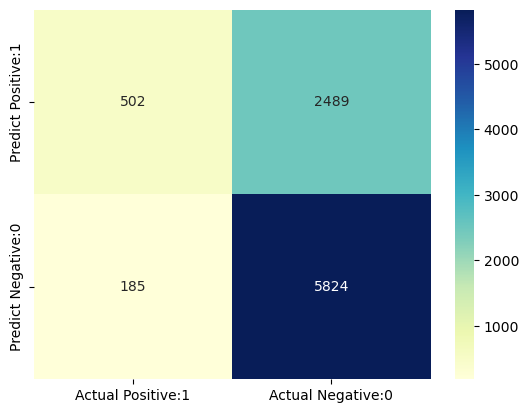
\includegraphics[width=0.5\textwidth]{BAB_TESIS/IMAGES/confusion_matrix.png}
	\caption{Confusion Matrix}
	\label{fig:confusion_matrix}
\end{figure}

\begin{table}[H]
	\caption{Confusion Matrix}
	\centering
	\begin{tabular}{|c|c|c|}
		\hline
		& \textbf{Predicted: 0} & \textbf{Predicted: 1} \\
		\hline
		\textbf{Actual: 0} & True Negative & False Positive \\
		\hline
		\textbf{Actual: 1} & False Negative & True Positive \\
		\hline
	\end{tabular}
	\label{table:1}
\end{table}

Hasil tertinggi yang diperoleh dari Tabel \ref{table:sampel_hasil_pengujian_random_forest} adalah sebagai berikut:

\begin{table}[H]
	\caption{Hasil Pengujian Random Forest}
	\centering
	\begin{tabular}{|c|c|}
		\hline
		\textbf{Parameter} & \textbf{Values} \\
		\hline
		n\_estimators & 500 \\
		\hline
		max\_depth & None \\
		\hline
		min\_samples\_split & 2 \\
		\hline
		min\_samples\_leaf & 2 \\
		\hline
	\end{tabular}
	\label{table:hasil_rf}
\end{table}

Dengan hasil sebagai akurasi 0.708, presisi 0.701, recall 0.968, dan F1 score 0.813. Dengan hasil ini diperoleh akurasi yang lebih rendah dari yang diharapkan. Hal ini disebabkan oleh dataset yang digunakan tidak seimbang. Dengan demikian, model yang dihasilkan cenderung memprediksi kelas mayoritas. Untuk membuktikan hal ini, dapat dilakukan pengecekan dengan melihat presentase target pada dataset. Berikut adalah presentase target pada dataset

	\section{Pembahasan Hasil Pengujian}
	\label{pembahasan hasil pengujian}
	Pembahasan hasil pengujian berisi pembahasan terhadap hasil pengujian yang telah dilakukan. Pembahasan dilakukan dengan membandingkan hasil pengujian dengan spesifikasi kebutuhan yang telah ditetapkan sebelumnya. Apabila hasil pengujian sesuai dengan spesifikasi kebutuhan, maka sistem dapat dikatakan berhasil. Sebaliknya, apabila hasil pengujian tidak sesuai dengan spesifikasi kebutuhan, maka sistem dapat dikatakan gagal.



%-----------------------------------------------------------------
% Akhir BAB 6
%-----------------------------------------------------------------


%-----------------------------------------------------------------
% Awal BAB 7
%-----------------------------------------------------------------
\chapter{KESIMPULAN DAN SARAN}
\label{kesimpulan dan saran}
Pada bagian ini dijelaskan mengenai kesimpulan dari penelitian yang telah dilakukan. Penjelasan dibagi menjadi beberapa bagian, yaitu kesimpulan, dan saran.

	\section{Kesimpulan}
	\label{penutup kesimpulan}
	Kesimpulan dari penelitian ini adalah sebagai berikut:
\begin{enumerate}
	\item Model yang dihasilkan belum dapat mengklasifikasi risiko autentikasi dengan baik. Sistem autentikasi M2M berbasis risiko menggunakan Random Forest dapat mengklasikasi risiko autentikasi. Dengan akurasi 70.8\%, presisi 70.1\%, \textit{recall} 96.8\%, dan \textit{F1-score} 71.3\%. Ketimpangan akurasi dan \textit{recall} disebabkan oleh ketidakseimbangan jumlah data pada kelas yang berbeda.
	\item Pembatasan fitur kepentingan dapat berpengaruh pada akurasi sistem.
\end{enumerate}


	\section{Saran}
	\label{penutup saran}
	Penelitian ini masih memiliki beberapa kekurangan yang dapat diperbaiki pada penelitian selanjutnya, yaitu:
\begin{enumerate}
	\item Penelitian ini masih menggunakan dataset hybrid. Sehingga perlu dilakukan penelitian lebih lanjut dengan menggunakan dataset asli.
	\item Akurasi sistem masih dapat ditingkatkan, serta perlu dilakukan penelitian lebih lanjut untuk meningkatkan keamanan sistem.
	\item Opitimasi parameter Random Forest masih dapat dilakukan lebih lanjut.
	\item Dapat dilakukan perbandingan dengan memilih target parameter yang berbeda.
\end{enumerate}


%-----------------------------------------------------------------
% Akhir BAB 7
%-----------------------------------------------------------------

%-----------------------------------------------------------------
% Awal Daftar Pustaka
%-----------------------------------------------------------------
\begin{thebibliography}{99}
    \addcontentsline{toc}{chapter}{DAFTAR PUSTAKA}
    
    \bibitem[Agarwal et al.(2016)]{Agarwal2016}
    Agarwal, L., Khan, H., \& Hengartner, U. (2016). Ask Me Again But Don’t Annoy Me: Evaluating Re-authentication Strategies for Smartphones. 221–236. \url{https://www.usenix.org/conference/soups2016/technical-sessions/presentation/agarwal}
    
    \bibitem[Alam \& Vuong(2013)]{Alam2013}
    Alam, M. S., \& Vuong, S. T. (2013). Random Forest Classification for Detecting Android Malware. 2013 IEEE International Conference on Green Computing and Communications and IEEE Internet of Things and IEEE Cyber, Physical and Social Computing, 663–669. \url{https://doi.org/10.1109/greencom-ithings-cpscom.2013.122}
    
    \bibitem[Cabarcos et al.(2019)]{Cabarcos2019}
    Cabarcos, P. A., Arias-Cabarcos, P., Krupitzer, C., \& Becker, C. (2019). A Survey on Adaptive Authentication. ACM Computing Surveys, 52(4), 80. \url{https://doi.org/10.1145/3336117}
    
    \bibitem[Doerfler et al.(2019)]{Doerfler2019}
    Doerfler, P., Thomas, K., Marincenko, M., Ranieri, J., Jiang, Y., Moscicki, A., \& McCoy, D. (2019). Evaluating Login Challenges as a Defense Against Account Takeover. 372–382. \url{https://doi.org/10.1145/3308558.3313481}
    
    \bibitem[Dutson et al.(2019)]{Dutson2019}
    Dutson, J., Allen, D., Eggett, D. L., \& Seamons, K. E. (2019). Don’t Punish all of us: Measuring User Attitudes about Two-Factor Authentication. 119–128. \url{https://doi.org/10.1109/eurospw.2019.00020}
    
    \bibitem[Braunstein(2022)]{Braunstein2022}
    Braunstein, Mark L. (2022). FHIR. Computers in Health Care, 233–291. \url{https://doi.org/10.1007/978-3-030-91563-6_9}
    
    \bibitem[Misbahuddin et al.(2017)]{Misbahuddin2017}
    Misbahuddin, M., B. S. Bindhumadhava, B. S. Bindhumadhava, Bindhumadhava, B. S., \& Dheeptha, B. (2017). Design of a risk-based authentication system using machine learning techniques. 1–6. \url{https://doi.org/10.1109/uic-atc.2017.8397628}
    
    \bibitem[Prasad et al.(2017)]{Prasad2017}
    Prasad, K. K., K, K. P., \& Aithal, S. (2017). A Study on Enhancing Mobile Banking Services Using Location Based Authentication. \url{https://doi.org/10.47992/ijmts.2581.6012.0006}
    
    \bibitem[Rahat et al.(2021)]{Rahat2021}
    Rahat, Tamjid Al, Feng, Yu, \& Tian, Yuan. (2021). Cerberus. Cornell University - ArXiv. \url{https://doi.org/10.1145/3548606.3559381}
    
    \bibitem[Roy \& Dasgupta(2018)]{Roy2018}
    Roy, A., \& Dasgupta, D. (2018). A fuzzy decision support system for multifactor authentication. Soft Computing - A Fusion of Foundations, Methodologies and Applications, 22(12), 3959–3981. \url{https://doi.org/10.1007/s00500-017-2607-6}
    
    \bibitem[Solapurkar(2016)]{Solapurkar2016}
    Solapurkar, P. (2016). Building secure healthcare services using OAuth 2.0 and JSON web token in IOT cloud scenario. International Conferences on Contemporary Computing and Informatics, 99–104. \url{https://doi.org/10.1109/ic3i.2016.7917942}
    
    \bibitem[Speiser et al.(2019)]{Speiser2019}
    Speiser, J. L., Miller, M., Miller, M. E., Tooze, J. A., \& Ip, E. H. (2019). A Comparison of Random Forest Variable Selection Methods for Classification Prediction Modeling. Expert Systems With Applications, 134, 93–101. \url{https://doi.org/10.1016/j.eswa.2019.05.028}
    
    \bibitem[Wiefling et al.(2021)]{Wiefling2021}
    Wiefling, Stephan, Markus Dürmuth, \& Luigi Lo Iacono. (2021). What’s in Score for Website Users: A Data-driven Long-term Study on Risk-based Authentication Characteristics. Financial Cryptography. \url{https://doi.org/10.1007/978-3-662-64331-0_19}
    
    \bibitem[Wiefling et al.(2022)]{Wiefling2022}
    Wiefling, Stephan, Paul René Jørgensen, Sigurd Thunem, \& Luigi Lo Iacono. (2022). Pump Up Password Security! Evaluating and Enhancing Risk-Based Authentication on a Real-World Large-Scale Online Service. ACM Transactions on Privacy and Security. \url{https://doi.org/10.1145/3546069}
    
    \bibitem[Taneja(2013)]{Taneja2013}
    Taneja, M. (2013). An analytics framework to detect compromised IoT devices using mobility behavior. Information and Communication Technology Convergence, 38–43. \url{https://doi.org/10.1109/ictc.2013.6675302}
    
    \bibitem[Thomas et al.(2017)]{Thomas2017}
    Thomas, K., Li, F., Zand, A., Barrett, J., Ranieri, J., Invernizzi, L., Markov, Y., Comanescu, O., Eranti, V., Moscicki, A., Margolis, D., Paxson, V., \& Bursztein, E. (2017). Data Breaches, Phishing, or Malware?: Understanding the Risks of Stolen Credentials. 1421–1434. \url{https://doi.org/10.1145/3133956.3134067}
    
    \bibitem[Zhang et al.(2012)]{Zhang2012}
    Zhang, F., Kondoro, A., \& Muftic, S. (2012). Location-Based Authentication and Authorization Using Smart Phones. 2012 IEEE 11th International Conference on Trust, Security and Privacy in Computing and Communications, 1285–1292. \url{https://doi.org/10.1109/trustcom.2012.198}
\end{thebibliography}

%-----------------------------------------------------------------
% Akhir Daftar Pustaka
%-----------------------------------------------------------------


%-----------------------------------------------------------------
% Awal lampiran
%-----------------------------------------------------------------
%\appendix

%\chapter{BERKAS JSON UNTUK MODEL SISTEM PENGENALAN ENTITAS BERNAMA}
%\label{BERKAS JSON UNTUK MODEL SISTEM PENGENALAN ENTITAS BERNAMA}
%\input{BAB_TESIS/BAB9_LAMPIRAN/1_BERKAS_MODEL_NER}

%-----------------------------------------------------------------
% Akhir lampiran
%-----------------------------------------------------------------

\end{document}